\chapter{時空間フェンシングに基づいたクラウドセンシングプラットフォーム}
\thispagestyle{myheadings}
本章ではまず時空間フェンシングの概念を定義し,時空間フェンシングに基づいたクラウドセンシングプラットフォーム「$\text{Lav.}^{+}$(ラヴラス)」を構築する.
3.1節では時空間フェンシングの定義を行い,時空間フェンシングによるクラウドセンシングの利点を述べる.
3.2節では時空間フェンシングに基づいたクラウドセンシングプラットフォームの要求仕様を述べる.
3.3節では本クラウドセンシングプラットフォームの手順を述べ,クラウドセンシングプラットフォームのサーバ,依頼者専用のWebアプリケーション(以下,Webアプリ),協力者専用のスマートフォンアプリケーション(以下,スマホアプリ)の実装について述べる.
3.4節では本プラットフォームの動作検証について述べる.


本クラウドセンシングプラットフォーム「$\text{Lav.}^{+}$」(以下,ラヴラス)の命名は,"a view of Laplace's demon"「ラプラスの魔の視界」から来ている.
ラプラスの魔とは,ピエール=シモン・ラプラスによって提唱された概念で「自然界のあらゆる力と宇宙全体のある時点における状態を完全に把握することができ,かつ,これらの素材を完璧に解析する能力をもった仮想的な知的存在.このような魔(demon)にとっては宇宙の中に何一つとして不確実なものはなく,未来のことを完璧な形で予見することが可能となる.」\cite{ziten}というものである.
本プラットフォームは,ラプラスの魔のコンセプトにちなんで,クラウドセンシングを用いて実世界の様相を把握し分析しラプラスの魔の視界を垣間見られる様なプラットフォームを目指すという意味を込めてラヴラスと命名した.
%

\section{時空間フェンシングの定義}

\begin{figure}[H]
    \centering
    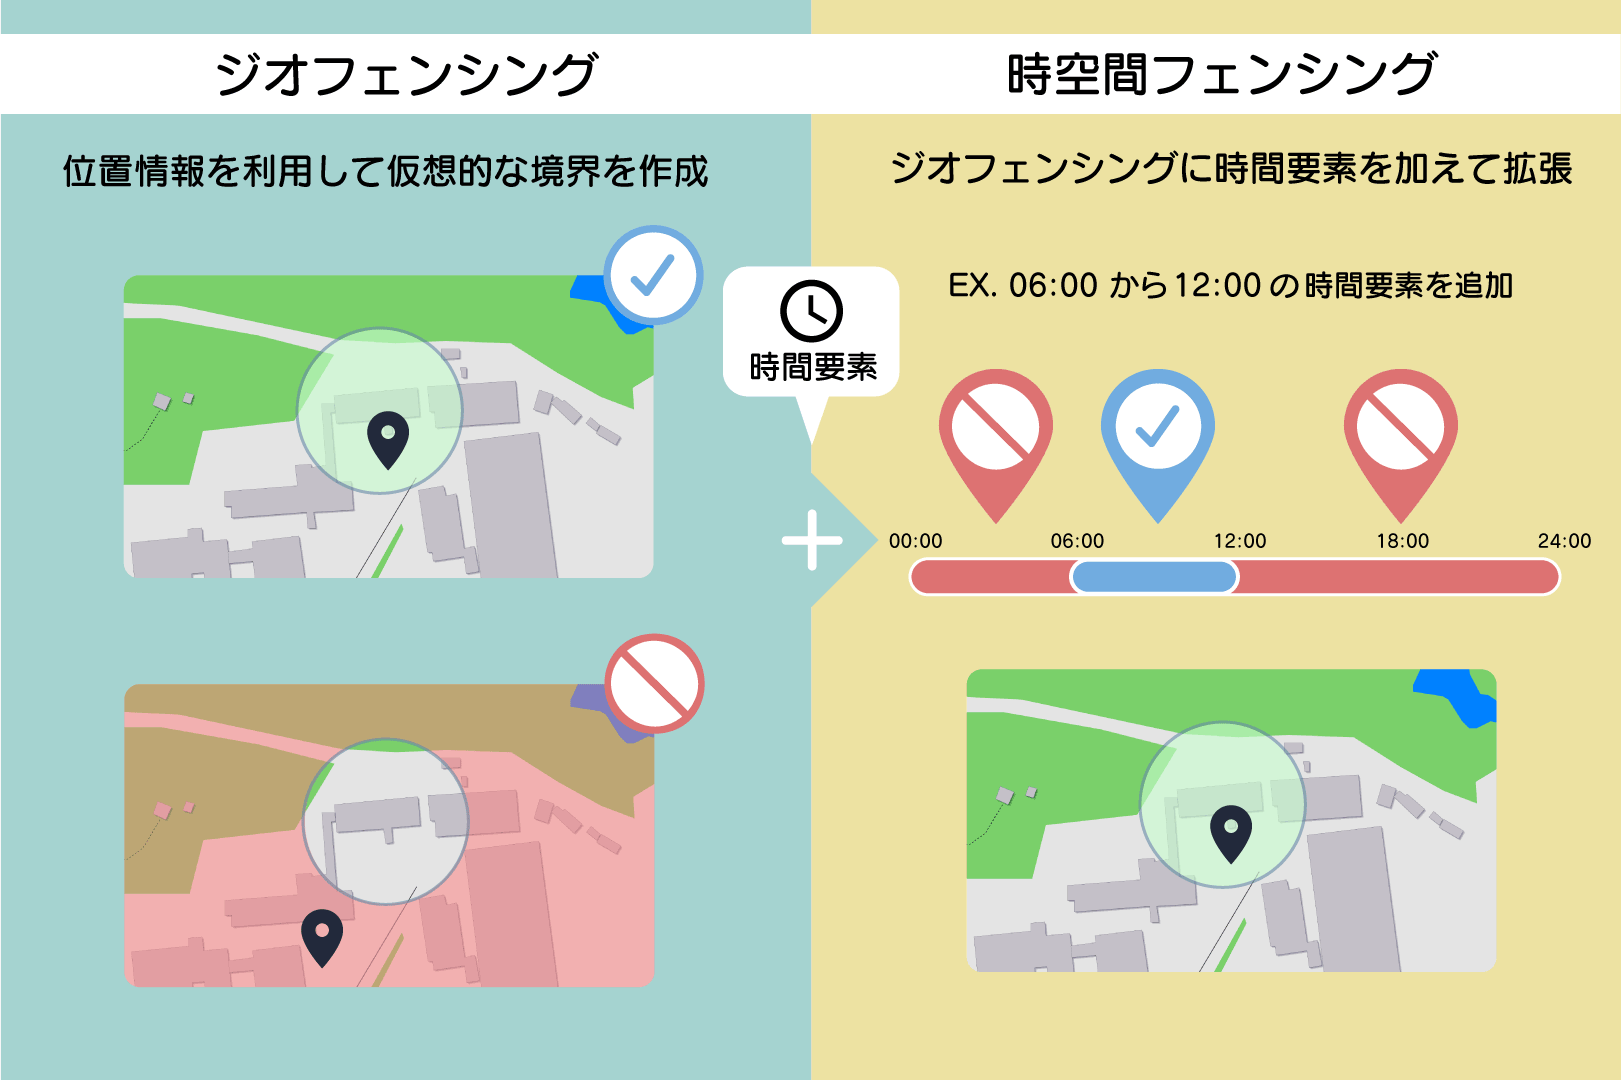
\includegraphics[width=150mm]{spatiotemporal.png}
    \caption{ジオフェンシングと時間要素を追加した時空間フェンシング}
    \label{fensing}
\end{figure}

時空間フェンシングは「ジオフェンシングに時間要素を追加し拡張したフェンシング手法」として定義する.
ジオフェンシングとはGPSやWi-Fi,BLEビーコンといった位置推定技術によって仮想的な境界を生成し,その境界に進入した,あるいは退出したときに特定のサービスを行うフェンシング手法である.
位置推定の高精度化や手軽にジオフェンスを構築できるBLEのようなデバイスの普及に伴って,ジオフェンシングを用いた様々なアプリケーションが実現されている.
つまり,時空間フェンシングとは,エリアと時間帯の指定によって仮想的な境界を生成し,その境界に進入した,あるいは退出したときに特定のサービスを行うフェンシング手法である.
特定のサービスとは,本研究では「センシング」である.
仮想的な境界内に進入したときにセンシングを開始し,境界外に退出したときにセンシングを終了する.

時空間フェンシングによって時間とエリアで境界を区切ると,依頼者は様々なシチュエーションを指定したクラウドセンシングが可能となる.
様々なシチュエーションとは,例えば「午後3時から5時の公園」であったり,「3限の1号館401教室」や「昼間の食堂」などである.
一方で,時空間フェンシングは時間やエリアに依存しないデータ収集には適さない.
例えば,一日中センシングを行なったり,電車で移動したりなどである.
このような長時間のセンシングやいつ終了するか定かではないセンシングは,協力者に消費電力など大きな負担をかけてしまう.
また,エリアのみ及び時間帯のみを指定するデータ収集には適さない.
エリアのみの場合,どこでセンシングされているかは分かっているが,いつセンシングされているかが明確ではない.
時間帯のみの場合も同様である.
依頼者と接点のない赤の他人が依頼者のセンシングに協力するとなった際,少しでもセンシング時間帯・エリアが曖昧であると,協力者は「協力しない」を選択する.
エリアと時間帯両方の明確な設定により,赤の他人のセンシングへの協力判断がしやすくする.
そのため本プラットフォームでは,依頼者が想定し得るすべてのセンシングに対応している訳ではない.
あくまでも時空間を指定したセンシングを想定している.

協力者のクラウドセンシングに対するプライバシ障壁は,時空間フェンシングによる時間とエリアの制限で軽減できる.
時間とエリアの指定がない場合,協力者は「いつどこでセンシングが開始し,終了するかわからない」という不安が生じるため,クラウドセンシングへの協力の判断がしにくい.
時間とエリアの指定がある場合,協力者は自分自身がプライベートな活動をしているのか,ある程度他人にデータ提供しても良い活動をしているのかを区別・判断しやすくなるため,クラウドセンシングへの協力の判断がしやすくなる.
時空間フェンシングにより,協力者は自分自身の可能な範囲内でセンシングに協力ができる.
% -----------------------------------------------
% -----------------------------------------------
% -----------------------------------------------

\section{ラヴラスの要求仕様}

本節では,ラヴラスにおける非機能要件を提示する.
3.2.1項では,ラヴラスにおけるクラウドセンシングプラットフォームとしての設計基盤について述べる.
3.2.2項では,協力者のプライバシ保護について述べ,3.2.3項では依頼者がラヴラスを利用する際の規約方針について述べる.
3.2.4項では,ラヴラスにおける利用者への配慮について述べる.
% -----------------------------------------------

\subsection{ラヴラスにおけるクラウドセンシングプラットフォームとしての設計基盤}
クラウドセンシングプラットフォームを構築するためには,一定の制限・制約を設計基盤として設ける必要がある.
この一定の制限・制約は,依頼者にとってクラウドセンシングの定義を簡略化でき,協力者にとっては受け入れやすいプラットフォームになるというメリットがある.
また,クラウドセンシングの実施方法に決まった手法や手順はなく,依頼者によって多種多様であるため,制限や制約はプラットフォームとして成立させるために必要不可欠な要素である.
関連研究として挙げた松田らの研究\cite{matsu}では,「ユーザ参加型モバイルセンシング基盤」という表現で我々のクラウドセンシングプラットフォームとしての設計基盤についての同様の記述がある.
松田らの研究では,ゲーミフィケーションによって協力者の協力へのモチベーションを向上させ,クラウドセンシングを行うための「シナリオ」がモジュール化されて定義されている.
それが我々のクラウドセンシングプラットフォームとしての設計基盤に相当する.
松田らの研究における「シナリオ」は,新規モジュールを開発し新たな「シナリオ」を追加はできるものの,モジュール化されていない「シナリオ」でのセンシングは出来ないという制約がある.

我々の構築するクラウドセンシングプラットフォーム「ラヴラス」のセンシングプラットフォームとしての設計基盤は,時空間フェンシングである.
我々が先ほど定義した時空間フェンシングを用いて,センシングを行う時間とエリアを制限するという制約を設けている.
時空間フェンシングをクラウドセンシングプラットフォームとしての設計基盤とすると,依頼者としては主に時空間フェンシングの設定とセンシングの設定の2つを定義すればいいため,容易にクラウドセンシングの定義が可能となる.
協力者としては,一定の時空間内でのみのセンシングであるため,プライバシの観点からクラウドセンシングへの協力を受け入れやすいといえる.

ラヴラスで実現しないセンシングは,時空間フェンシングでは適さないセンシングである.
例えば,一定の時間に依存しない1日の運動量といった長時間に渡るセンシングや時間に制限のない一定エリアでの活動のすべてといったセンシング,空間に依存しない車や電車等での移動中といったセンシングである.
これらは時空間内でのみセンシングという制限により,ラヴラスでは行わない.
また,時空間フェンシングの最大範囲を制限し,ラヴラスが定義する時間やエリアの範囲を超える時空間は定義できない.
これはエリアが市や県単位であったり,時間が「0時から24時」であった場合,制限がないのと同じになってしまうからである.
% -----------------------------------------------

\subsection{プライバシの保護}
世界的なインターネットの一般化によって,インターネットサービスを利用する際の個人データの取り扱いが重要となっている.
例えば,Facebookでは個人情報の不正流出が問題となり,2018年4月10日にCEOであるマーク・ザッカーバーグ氏が謝罪を行っている\cite{facebook}.
このような背景から,EUは個人データの取り扱いに対して,2018年5月25日にデータ保護指令(Data Protection Directive)に変わるGDPR(General Data Protection Regulation:一般データ保護規則)\cite{GDPR}を施行した.
GDPRは個人データやプライバシーの保護に関して,データ保護指令より厳格に規定し,制裁も強化している.

こういった国際的動向から,ラヴラスにおいてもプライバシの保護は必須である.
まず,設計基盤である時空間フェンシングという制限によって,時間やエリアの指定がないセンシングを実施しない.
また,時間やエリアを指定されている場合でも,依頼者の承諾なしでのセンシングは行わない.
これらにより,協力者の意図しないセンサのログデータ(以下,センシングデータ)の提供に伴うプライバシの侵害というリスクを最小限に抑える.
加えて,各協力者から提供されるセンシングデータやそれに結びつく端末情報などのセンシティブな情報を取り扱うため,依頼者のユーザ認証により,第三者による意図しないアクセスや情報の改ざんなどを防ぐ.

GDPRの個人データの定義(第4条)によると,協力者から提供される各センシングデータそのものは個人データには分類されないとされている.
しかし,そのセンシングデータに付随される情報との組み合わせによって,個人データに分類される可能性がある.
そのため,ラヴラスにはセンシングデータが個人情報となりえない設計が必要である.
例えば,協力者からのセンシングデータ提供の際,センシング行った環境情報として端末名やセンサの型番などの端末情報(以下,メタデータ)を取得するが,端末識別IDであるIMEI(International Mobile Equipment Identity)は個人データとなるため取得しない.
加えて,メタデータにはIMEI以外に,センシングデータとメタデータの参照により個人が識別可能になる場合,メタデータはセンシングを行った環境が判明する情報のみ取得するものとする.

さらに,協力者が特定のセンシングを拒否できる設計や提供したデータの削除要請を行う機能が必要がある.
上記で述べたように協力者から提供されるセンシングデータ及びメタデータは,個人情報に繋がらない特性情報のみに留めている.
しかし,協力者がプライバシを侵害されていると感じた場合,協力者の都合により特定のセンシングの拒否及び提供済みのセンシングデータ削除の要請などの要求に対応しなければならない.
依頼者側は協力者の協力拒否や削除要請の拒絶はできない.
これは,クラウドセンシングとは協力者ありきのデータ収集方法であり,協力者の信頼をなくしてしまっては成り立たないからである.
もし拒絶ができた場合,クラウドセンシングに対する信頼はなくなってしまい,協力者は該当のセンシングだけではなく,本プラットフォームの利用をやめてしまう可能性がある.
% 本プラットフォームは関連研究で述べたようなインセンティブを用いていないため,より協力者を第一に考えるプラットフォームでなければならない.
% -----------------------------------------------

\subsection{ラヴラスの利用規約方針}
依頼者はラヴラスを利用してクラウドセンシングを行う際,センシングの依頼(以下,センシングプロジェクト)を作成する必要がある.
センシングプロジェクトの作成を行うためには,依頼者の利用資格とそのセンシングプロジェクトを立ち上げる目的や使用センサ等のセンシングプロジェクトの内容の明示が必要である.
依頼者の利用資格を得るには,依頼者自身の情報が明示されている必要があり,匿名によるセンシングプロジェクトの作成はできない.
この依頼者情報は,基本的に依頼者本人の責任で保証されるものとし,ラヴラスでは登録されるメールアドレスが大学や所属機関のものかどうかなどの簡易的な確認のみを行うものとする.
センシングプロジェクトの内容の明示では,そのセンシングがどんな目的で行われるのか,センサはどんなものを使用するのか,実施期間や時空間フェンシングといった依頼内容を定義したものを明示する.
これは,どんな依頼者がどんな目的でデータ収集したいのかを明確にし,その実施内容が妥当なものであるのかを協力者が判断ができるようにするために必要である.
該当のセンシングプロジェクトの協力者にこれらの情報を明示し,協力者はその内容を了承した上でセンシングプロジェクトに協力する.

センシングデータの取り扱いの禁止事項として,「センシングデータの再利用禁止」と「保存期間以上のセンシングデータの保存禁止」を制定する.
センシングデータの再利用禁止は,「センシングデータの利用は依頼者本人(組織の場合はその組織)のみであるものとし,依頼者は収集したセンシングデータをそのプロジェクトに明示した目的を超える利用や第三者への開示・譲渡等は禁止する」と示す.
これは,協力者が依頼者のセンシングプロジェクトに同意した上で提供したセンシングデータが,協力者の意図と反して利用されてしまうからである.
ラヴラスが指定する保存期間以上のセンシングデータの保存の禁止は,「ラヴラスが定めるセンシングデータの保存期間を超える長期間の保存は禁止とする」と示す.
これは,センシングデータの提供方法をダウンロードとしているため,3.2.2項で述べた協力者による提供済みのセンシングデータの削除要請によって,削除されたセンシングデータが適切に利用できなくなるようにするためである.
センシングデータの提供方法をダウンロードとしているのは,依頼者が独自の環境で柔軟にセンシングデータの解析が行えるようにサポートするためである.
協力者による提供済みのセンシングデータの削除要請が行われたとき,直ちにサーバに保存された該当のセンシングデータの削除が行われるものとする.
しかし,削除要請以前に該当のセンシングデータが依頼者によってダウンロードされ,保存期間の終了前であった場合は,依頼者に該当のセンシングデータが削除要請によってサーバから削除されたと通知し,直ちに該当のセンシングデータの利用中止・削除を要請する.
このとき協力者の削除要請から依頼者が利用できなくなるまでにラグの発生が予想されるため,協力者に利用規約として提供済みのセンシングデータの削除要請が直ちに実行されるものではないと事前に通知する.
% -----------------------------------------------

\subsection{利用者への配慮}
ラヴラスの利用過程において負担となる要素がある場合,利用者は獲得しにくくなる.
そのため,利用者の視点から快適に利用できると思える配慮が必要である.
こうした配慮は,依頼者・協力者共に受け入れやすいプラットフォームを実現するために必要であり,依頼者と協力者が相互に利用しやすいプラットフォームを目指す上で重要となる.
本節では,心理的負担と物理的負担の2つの視点に分けて,その負担と配慮について述べる.

心理的負担としては,協力者がクラウドセンシングに協力する際に抱くプライバシを侵害されているという不安が挙げられる.
これは,協力者にとってスマートフォンから意図しないセンシングデータが提供されるかもしれないという不安ともいえる.
これに対する配慮として,安心してクラウドセンシングに協力できる環境を提案する必要がある.
まず,3.2.1項で挙げた時空間フェンシングによる時間とエリアによる制限がある.
協力者には,センシングプロジェクトに定義された時空間に進入した際にセンシングプロジェクトに協力するか否かを問う通知を送る.
協力者は,依頼内容や設定された時空間を確認した上で協力するかを判断し承諾された場合のみセンシングを行い,拒否した場合はセンシングは行わない.
このプロセスによって,協力者は意図したセンシングプロジェクトのみにセンシングデータの提供が可能である.
さらに,3.2.2項に挙げたように状況に応じてこのプロセスを通して承諾済みのセンシングプロジェクトの承諾取り消しや提供済みセンシングデータの削除が可能なため,誤って許可してしまったセンシングプロジェクトへの拒否や意図せず提供してしまったセンシングデータを削除もできる.

物理的な負担としては,1回のセンシング協力に伴う協力者の手間が挙げられる.
1回のセンシング協力にかかる手間が大きいほど,協力者のセンシング協力に対するモチベーションは低下し,継続的なセンシング協力は得られにくい.
これに対する配慮として,協力者の手間となるスマホアプリの操作は,基本的に上記に記した通知画面よりセンシングプロジェクトへの承諾及び拒否を行うのみで行えるように設計する.
この操作は協力するセンシングプロジェクトごとに初めの1回のみであるため,再度同じセンシングプロジェクトに設定された時空間に進入した場合は一切操作は行う必要はなく,自動的にセンシングを開始する.
また,センシングの終了や終了後のセンシングデータのアップロードは自動で行われるため,協力者がスマホアプリを操作する必要はない.
さらに,センシングデータのアップロードはWi-Fi環境下のみで行うため,協力者のパケット通信量を最小限に抑える.
この他に,依頼者・協力者に共通してラヴラスを利用する際に必要不可欠なユーザインターフェイスについても配慮を行う.
ユーザインターフェイスは,利用者によって使いやすさに直結するものである.
情報の表示や入力のしやすさが低ければ,利用者によって物理的負担となり利用されにくいプラットフォームとなるためである.
% -----------------------------------------------
% -----------------------------------------------
% -----------------------------------------------
% -----------------------------------------------

\section{ラヴラスの実装}
先述のプラットフォームの要求仕様に則って,クラウドセンシングプラットフォーム「ラヴラス」の実装を行う.
本プラットフォームは,センシングデータの管理や各プロジェクトを管理するサーバ,依頼者専用のプロジェクトの作成・管理を行うWebアプリ,協力者専用のセンシングを行うスマホアプリによって構成する.
3.3.1項では,依頼者と協力者がラヴラスを操作する際の手順について述べる.
3.3.2項では,センシングデータの管理や各プロジェクトを管理するサーバの実装について述べる.
3.3.3項では,依頼者専用のセンシングプロジェクト管理やセンシングデータダウンロードを行うWebアプリの実装について述べる.
3.3.4項では,協力者専用のセンシングスマホアプリの実装について述べる.
% -----------------------------------------------


\subsection{ラヴラスの操作手順}

\begin{figure}[H]
    \centering
    \includegraphics[width=150mm]{fig1.png}
    \caption{ラヴラスによるクラウドセンシングの操作手順}
    \label{fig:1}
\end{figure}

ラヴラスの一連の流れは「Webアプリでセンシングプロジェクトの定義」,「時空間フェンシング」,「センシング依頼の承諾」,「自動的にセンシング」,「Wi-Fi環境下で自動的にアップロード」,「データ利用」の順で行う(図\ref{fig:1}).
依頼者側では「Webアプリでセンシングプロジェクトの定義」と「データ利用」が行われる.
一方で,協力者側では「時空間フェンシング」,「センシング依頼の承諾」,「自動的にセンシング」,「Wi-Fi環境下で自動的にアップロード」が行われる.
ラヴラスを利用してクラウドセンシングを行う際のユーザの使用デバイスとして,依頼者はPCを,協力者はスマートフォンを前提としている.
依頼者がラヴラスを利用するためには,まずWebアプリでユーザ登録してもらう.
協力者がラヴラスのクラウドセンシングに協力するためには,ラヴラス専用のスマホアプリをインストールしてもらう.

依頼者はプロジェクト管理Webアプリにて,センシング依頼の内容を細かく定義し,センシングプロジェクトを作成する.
センシングプロジェクトとはセンシングを行いたい時間帯やエリア,センシングを行う目的,概要,センシングに用いるセンサの種類やそのセンサのサンプリングレートなどである.
これは協力者側のスマホアプリでセンシングや時空間フェンシングの設定に必要であるとともに,協力者にセンシングプロジェクトを提示し,協力するか否かの判断材料にしてもらう.
作成されたセンシングプロジェクトはスマホアプリ側が適宜取得し,取得したプロジェクトに応じて時空間フェンシング・センシング依頼通知・センシングを行う.

スマホアプリ側ではセンシングプロジェクトに応じて,3.1節の定義をもとに時空間フェンシングを行い,協力者が指定された時間帯かつエリアにいる場合のみ通知が送られる.
そのため,時間帯・エリアのどちらか一方のみ当てはまる場合は通知は送られない.
例えば,指定エリア内に進入していたとしても,指定時間帯に入っていない及び過ぎている場合は通知は送られない.
指定時間帯に入っていて,指定エリア内に進入していない場合も同様である.
また,時空間フェンシングはバックグラウンドで行うため,本スマホアプリを開いておく必要はない.
そして,指定された開始時間から終了時間の間であれば,いつ指定されたエリアに進入しても通知は送られる.
指定されたエリアを退出し,一定時間後再び進入した場合は,通知を送らずにセンシングを開始する.

\begin{figure}[H]
  \centering
  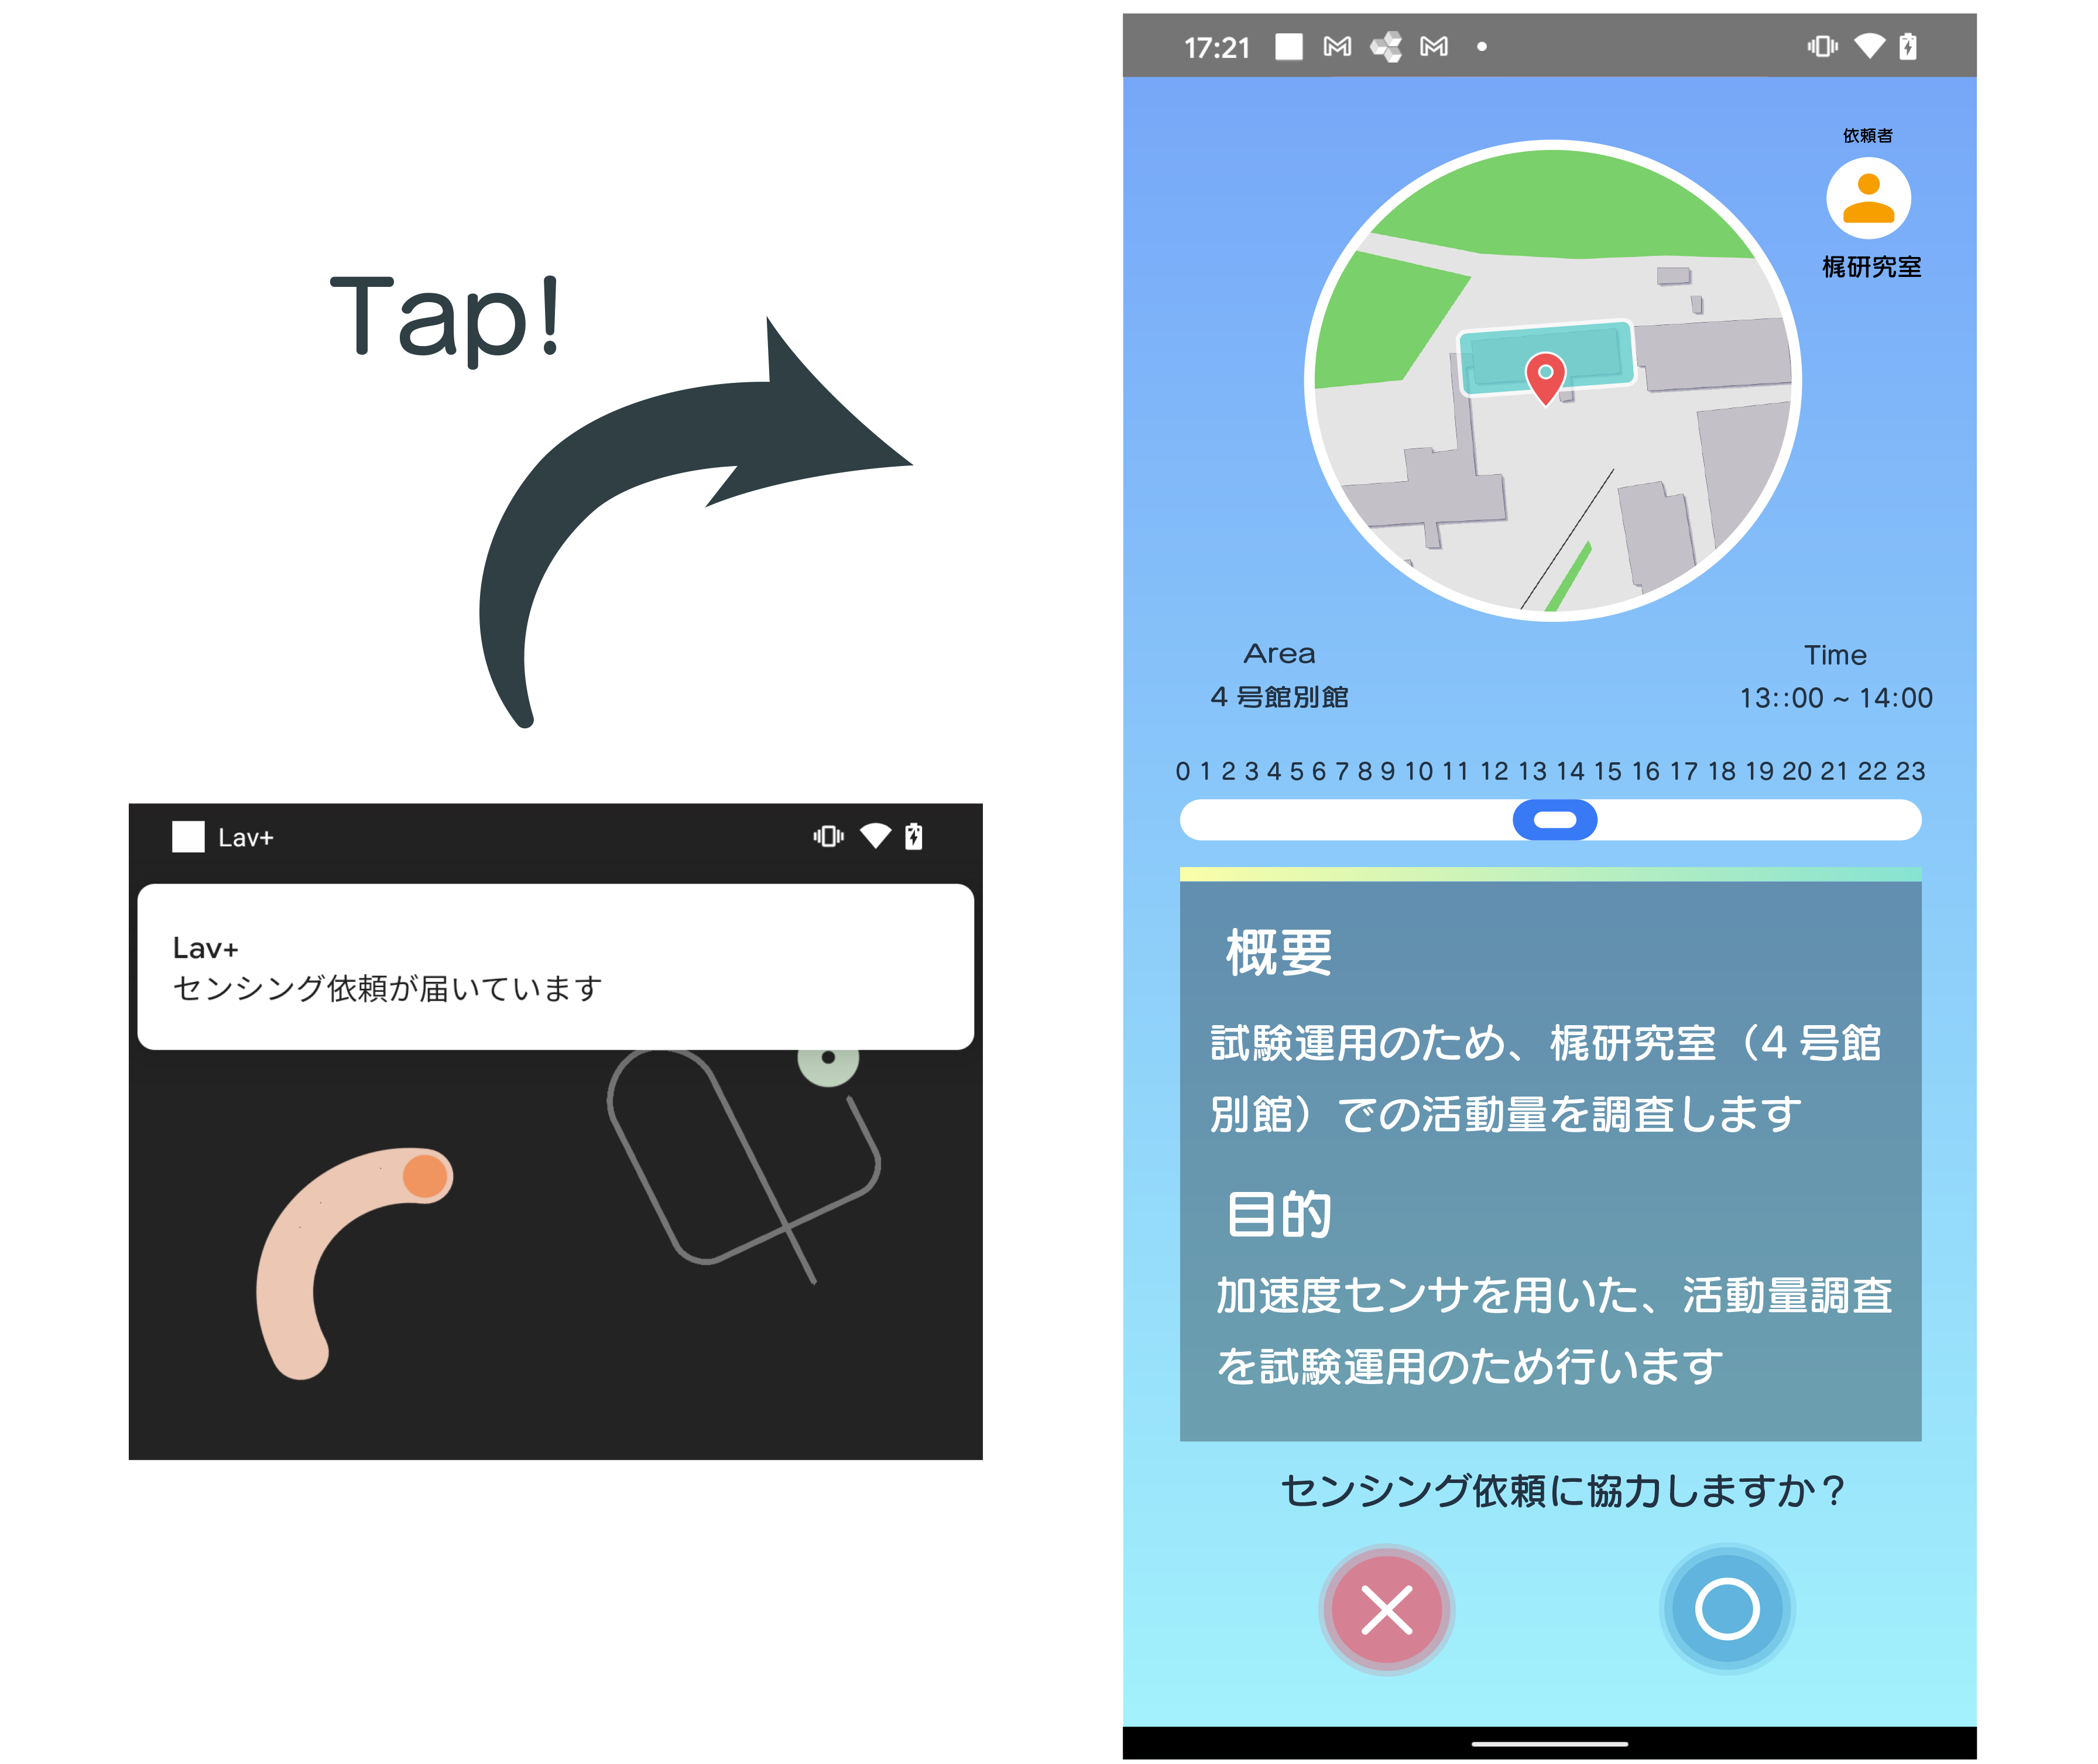
\includegraphics[width=100mm]{fig2.png}
  \caption{センシング依頼のヘッドアップ通知と通知画面}
  \label{fig:2}
\end{figure}

協力者はヘッドアップ通知のクリックで本アプリケーションの通知画面を開き,依頼されているセンシングプロジェクトの内容を確認し,承諾・拒否の判断をする.
通知画面で表示する情報としては,センシングを行うエリア,時間帯,センシングの目的,概要,依頼者の情報である.
また,時空間内に進入した際の現在地と指定エリアをGoogle Mapsで位置関係をより分かりやすく表示している.
センシング依頼の内容に納得し,協力してもいい場合に承諾ボタン(通知画面では丸ボタン)を押す.
そうすると,センシングが開始される.
通知が届いた時間帯やエリアが協力者にとってセンシングされたくない時間またはエリアの場合,または届いたセンシング依頼に協力したくない場合は,拒否ボタン(通知画面ではバツボタン) を押す.
そうすると,センシングは開始せずに終了する.
ラヴラスのクラウドセンシングの手順において協力者がスマートフォンを操作するのは主にこの通知から承諾・拒否の部分である.
承諾ボタンを押したら,もうスマホアプリは閉じても構わない.

センシングも常にバックグラウンドで行うため,アプリケーションを開いておく必要はない.
バックグラウンドでのセンシングにより,協力者がセンシング終了するなどの操作をする必要がない.
センシング終了後はWi-Fi接続時にのみ自動でサーバ側にアップロードされる.
協力者のスマートフォンがWi-Fiなどに接続されている場合にセンシングデータをサーバにアップロードする.
接続されていない場合は,アップロードせずディレクトリに格納しておき,Wi-Fiなどに接続された際にまとめてアップロードする.

依頼者は本Webアプリにて,アップロードされたセンシングデータを閲覧可能である.
% -----------------------------------------------

\subsection{センシングデータの管理や各プロジェクトを管理するサーバの実装}

センシングデータの管理や各プロジェクトを管理するサーバは,Webアプリ及びスマホアプリのどちらからの連携もスムーズ行えるようにそのどちらにも親和性が高いJSONベースのREST APIとして設計した.
REST APIとしてサーバを設計すると,MVCモデルにおけるModelとControllerをView部分にあたるWebアプリとスマホアプリを完全に分離し,実装の分業化及びオブジェクト指向設計の原則における単一責任の原則によって,各機能のカプセル化を実現し,メンテナンスや拡張実装をより柔軟にするという狙いもある.
サーバは,構築する上でJSON形式のファイルを取り扱いやすい言語を選択する必要があったため,JavaScript(Node.js)を選択した.
また,JavaScriptはJSONファイルをよりネイティブに取り扱いやすい言語であり,REST API専用のフレームワークの選択肢が他言語に比べて多く存在している.
REST APIのフレームワークは,Webサーバ系フレームワークとして有名なExpressを,REST API専用のフレームワークとして再設計されたLoopBack4を採用した.
サーバで使用するデータベースは,今後のスマートフォンのさらなる高性能化による搭載センサの種類増加に伴うデータベースの変更やシステムの拡張性の向上を図るため,変更や操作が柔軟に可能なデータベースとしてNoSQLデータベースのMongoDBを採用した.

サーバのデータベースとREST APIのエンドポイントを3.2節「ラヴラスの要求仕様」を基に設計を行った.
NoSQLデータベースであるMongoDBにはリレーショナルデータベースにおけるテーブルのカラムの概念が存在しないため,各モデルの定義をLoopBack4のモデルによって定義する.
以下の各モデルの説明には,LoopBack4で定義したモデルによって作成したコレクション(リレーショナルデータベースにおけるテーブルに相当)とそのコレクション内のドキュメント(リレーショナルデータベースにおけるレコードに相当)の一例を示すものとする.

\begin{figure}[H]
  \centering
  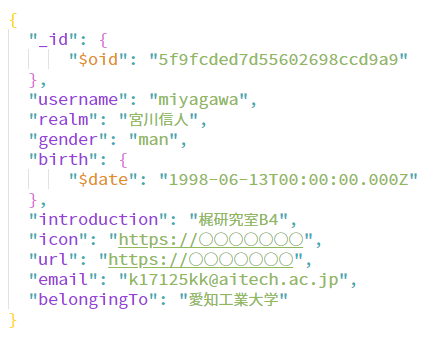
\includegraphics[width=96mm]{User.png}
  \caption{Userコレクションのドキュメント一例}
  \label{User}
\end{figure}

各依頼者を管理するためのモデルとしてUserモデル(図\ref{User})を定義した.
Userモデルには,ドキュメント管理用の「id」,ユーザ名「username」,依頼者の本名「realm」,性別「gender」,生年月日「birth」,紹介文「introduction」,アイコン画像「icon」,eメールアドレス「email」,Webページリンク「url」,所属機関「belongingTo」の10項目を定義した.
要求仕様の3.2.3項「ラヴラスの利用及び利用規約の方針」に基づき,依頼者の利用資格の観点から匿名によるセンシングプロジェクトの作成はできないため,ユーザ名,依頼者の本名,性別,生年月日,eメールアドレス,所属機関を必須項目として設定を行った.
REST APIのエンドポイントは,ユーザ登録を行う「/singup(POST)」,ログイン用の「/users/login(POST)」,ログイン後自身の情報を取得する「/whoAmI(GET)」を作成した.

\begin{figure}[H]
  \centering
  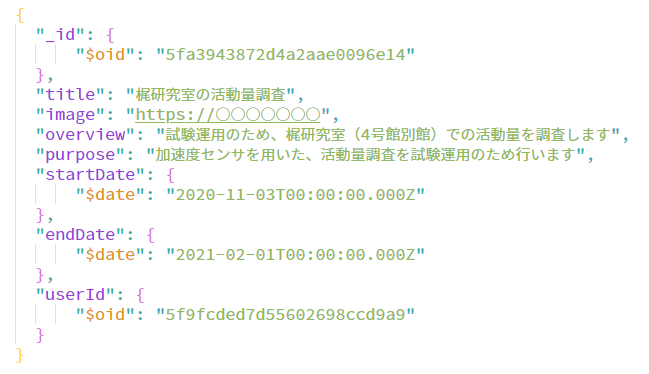
\includegraphics[width=120mm]{Project.png}
  \caption{Projectコレクションのドキュメント一例}
  \label{Project}
\end{figure}

各センシングプロジェクトを管理するためのモデルとしてProjectモデル(図\ref{Project})を定義した.
Projectモデルには,ドキュメント管理用の「id」,プロジェクトタイトル「title」,サムネイル用画像「image」,概要説明「overview」,目的「purpose」,センシングプロジェクトの開始日「startDate」と終了日「endDate」,作成したUserのid「userId」の8項目を定義した.
REST APIのエンドポイントは,「/project」でそれぞれの操作に対応するHTTPメソッドによりCRUD操作(Create,Read,Update,Delete)が可能となる.
これらの項目のうちサムネイル用画像以外の項目はすべて必須項目であり,要求仕様の3.2.3項「ラヴラスの利用及び利用規約の方針」に基づき,センシングプロジェクトの内容を明確にするために概要や目的の説明文の項目を定義している.
また,同要求仕様に示されたセンシングに関するセンサの定義や時空間フェンシングの定義は,SensingSettingモデルで定義を行っている.
センシングプロジェクト作成に必要な情報をProjectモデルとSensingSettingモデルに分離するのは,スマホアプリがSensingSettingモデルのエンドポイントから各センシングプロジェクトのセンシングに関する設定を直接的な読み込みを可能にするためである.

\begin{figure}[H]
  \centering
  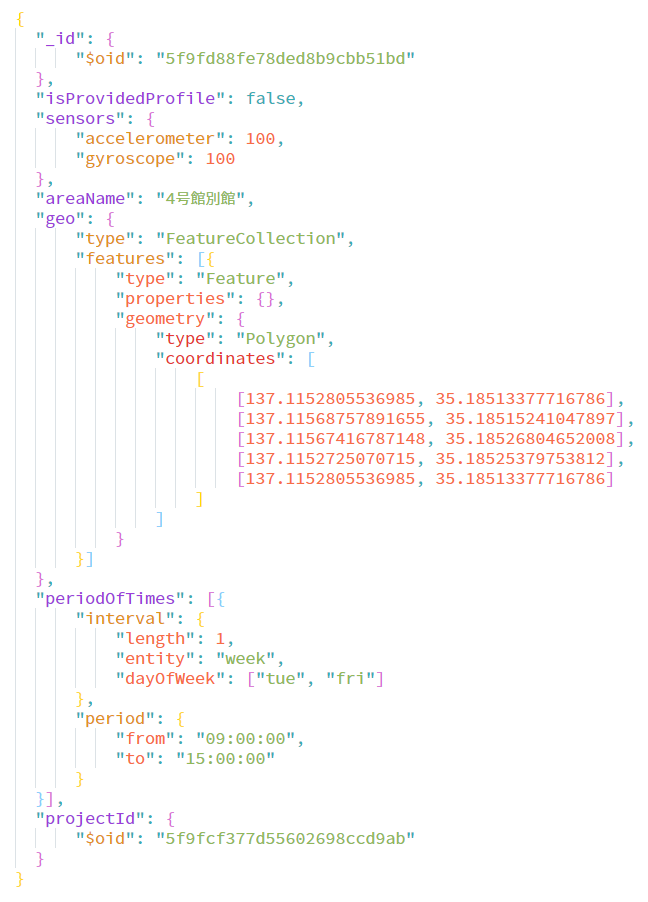
\includegraphics[width=120mm]{SensingSetting.png}
  \caption{SensingSettingコレクションのドキュメント一例}
  \label{SensingSetting}
\end{figure}

SensingSettingモデル(図\ref{SensingSetting})には,ドキュメント管理用の「id」,協力者に自身の基礎情報(身長・体重・性別など)を求めるか否かの設定「isProvidedProfile」,使用センサの種類とそれぞれのセンサのサンプリングレート(Hz)「sensors」,時空間フェンシングのエリア名「areaName」,GeoJSONによる時空間フェンシングのエリア設定「geo」,時空間フェンシングの時間帯設定「periodOfTimes」,紐づくセンシングプロジェクトのid「projectId」の7項目を定義した.
REST APIのエンドポイントは,「/sensing-setting」でそれぞれの操作に対応するHTTPメソッドによりCRUD操作が可能となる.
協力者に自身の基礎情報を求めるか否かの設定「isProvidedProfile」は,依頼者がセンシング協力を行う協力者の体格や性別に応じた変化を含めて調査を行いたい場合に利用するための項目として定義した.
これは,協力者に基礎情報の登録をスマホアプリで行ってもらい,その情報をセンシングデータと共に送信するものであるが,現在実装には至っていないため定義のみとする.
時空間フェンシングの定義として,柔軟に依頼者の想定するシチュエーションに対応するためには,複数のエリアや異なる時間帯を定義できるフォーマットにする必要がある.
時空間フェンシングのエリア設定「geo」は,現在のエリア判定方法がGPS情報による判定でのみであるため,地理的データを表現するフォーマットであるGeoJSON形式を用いてエリアの設定を行っている.
エリアの定義にGeoJSON形式を用いた理由は,2つ以上のエリアの定義を可能にできる他,複雑なエリアの指定も可能にするためである.

\begin{figure}[H]
  \centering
  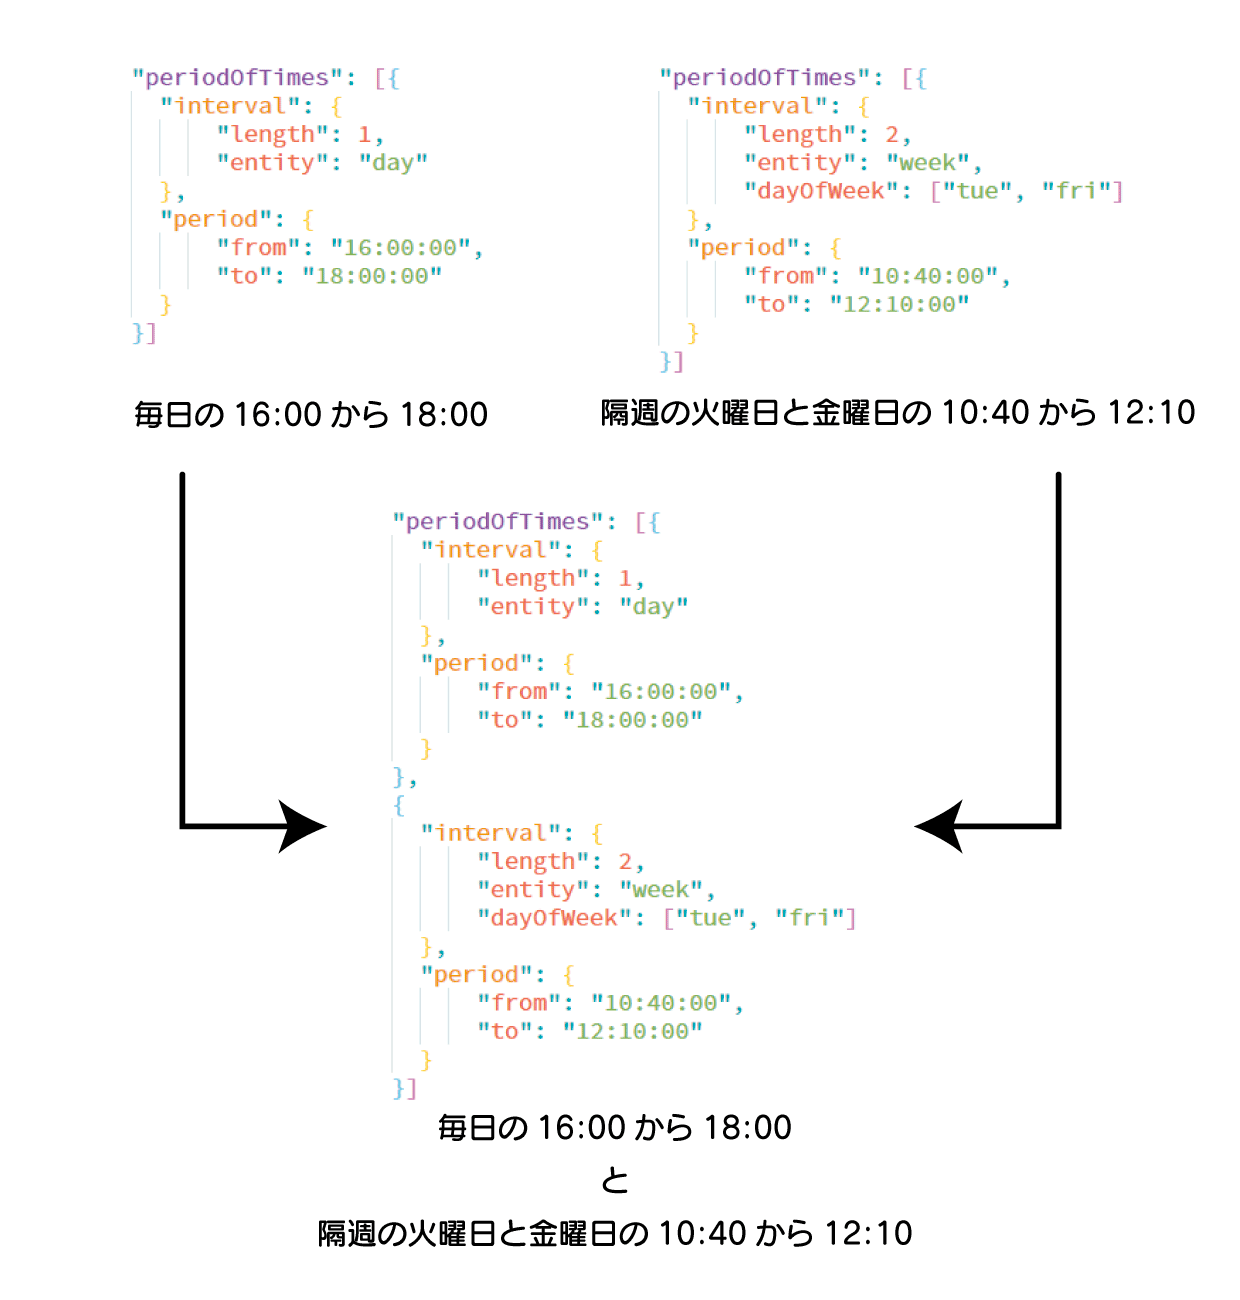
\includegraphics[width=150mm]{periodOfTimes.png}
  \caption{periodOfTimesの定義の例}
  \label{periodOfTimes}
\end{figure}

時空間フェンシングの時間設定「periodOfTimes」も,複数の時間帯を定義可能なフォーマットを定義した(図\ref{periodOfTimes}).
このフォーマットは,intervalとperiodからなるオブジェクトの配列として定義する.
intervalは,指定された時間帯を繰り返す間隔を定義するプロパティでlength,entity,dayOfWeekからなるオブジェクトである.
entityとdayOfWeekは間隔を設ける単位を表現し,entityには"day"もしくは"week"のどちらかのテキストが入り,"day"の場合はdayOfWeekプロパティが省略され,"week"の場合はdayOfWeekプロパティに指定する曜日を3文字の曜日の省略表記を用いて文字列の配列として定義する.
lengthには,数字を指定しentityとdayOfWeekで指定した単位で間隔を設ける.
periodは,fromプロパティにセンシング開始時間,toプロパティにセンシング終了時間を指定する.
このフォーマットによって例えば,「毎日の16:00から18:00まで」や「隔週の火曜日と金曜日の10:40から12:10」といった指定やその両方の指定が可能になる.

\begin{figure}[H]
  \centering
  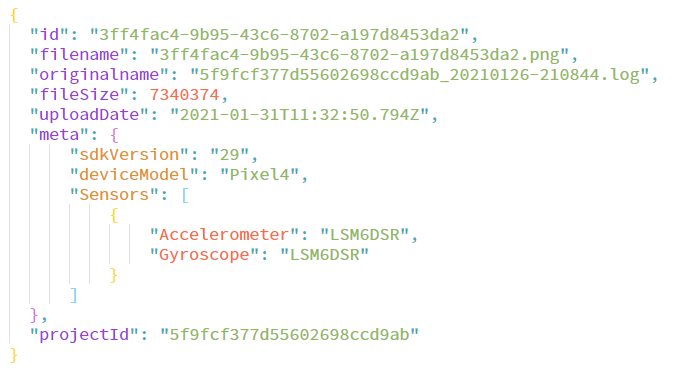
\includegraphics[width=120mm]{SensingData.png}
  \caption{SensingDataコレクションのドキュメント一例}
  \label{SensingData}
\end{figure}

協力者によって提供される各センシングデータを管理するモデルとしてSensingDataモデル(図\ref{SensingData})を定義した.
SensingDataモデルには,ドキュメント管理用の「id」,サーバ内部で保存したファイル名「filename」,協力者から提供されたオリジナルのファイル名「originalname」,ファイルのサイズ(byte)「fileSize」,アップロードが行われた日時「uploadDate」,メタデータ「meta」,提供されたセンシングプロジェクトのid「projectId」の7項目を定義した.
REST APIのエンドポイントは,「/sensing-data」でそれぞれの操作に対応するHTTPメソッドによりCRUD操作が可能となる.
オリジナルのファイル名を変更しサーバで保存を行っているのは,サーバ内で同名のファイルが保存され上書きされる可能性があるためである.
また,メタデータは要求仕様の3.2.2項「プライバシの保護」に基づき,個人データに該当しないOSのSDKバージョン,デバイスモデル,使用したセンサとその型番のみを取得する.
センシングデータをアップロードするための専用のエンドポイントとして,「/sensing-data/upload(POST)」を作成する.
このエンドポイントは,バイナリデータであるセンシングデータを取り扱うためにJSON形式によるエンドポイントではなく,「multipart/form-data」を使用し,スマホアプリがセンシングデータのアップロードと「/sensing-data」を通してセンシングデータの情報のアップロードを行う手間を削減するために,センシングデータがアップロードされるとサーバは自動的にSensingDataコレクションにドキュメントを作成する.

\begin{figure}[H]
  \centering
  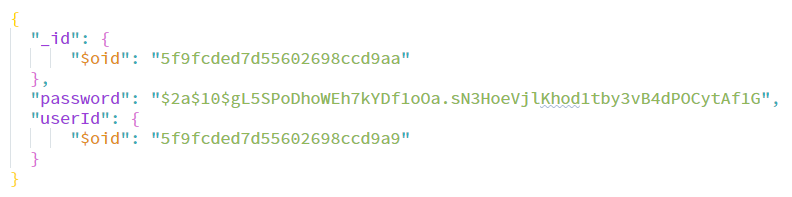
\includegraphics[width=150mm]{UserCredentials.png}
  \caption{UserCredentialsコレクションのドキュメント一例}
  \label{UserCredentials}
\end{figure}


最後に,要求仕様の3.2.2項「プライバシの保護」に対応するためのセキュリティ対策としてJWTトークン認証を導入した.
JWTトークン認証を実現するために,Userモデルに結びつき認証情報を保持するUserCredentialsモデル(図\ref{UserCredentials})を定義した.
UserCredentialsモデルには,ドキュメント管理用の「id」,依頼者が設定したパスワードのハッシュ値「password」,結びつくUserモデルのid「userId」の3項目で定義される.
セキュリティ対策として依頼者の設定したパスワードは,そのままの値で保持せずハッシュ値を用いている.
このJWTトークン認証によって各エンドポイントの不正なアクセスの防止を実現する.
例えば,提供済みのセンシングデータのダウンロードを行うエンドポイントは,センシングプロジェクトの作成を行った依頼者本人でなければアクセスができない.
図\ref{fig401}は,権限の無いユーザがセンシングデータのダウンロードを行うためのエンドポイントにアクセスした際に表示されるエラーメッセージである.



\begin{figure}[H]
  \centering
  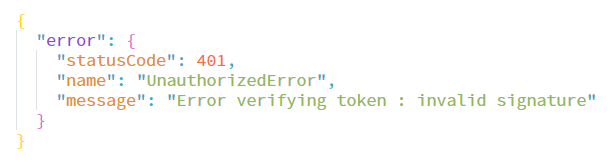
\includegraphics[width=120mm]{401.png}
  \caption{権限の無いユーザがセンシングデータのダウンロードを試みる例}
  \label{fig401}
\end{figure}

% -----------------------------------------------

\subsection{依頼者用のプロジェクト管理Webアプリの実装}

\begin{figure}[H]
  \centering
  \includegraphics[width= 150mm]{serverAndWeb.png}
  \caption{サーバとWebアプリの連携}
  \label{kanri}
\end{figure}

依頼者のユーザ登録やセンシングプロジェクトの作成及び管理を行うためのWebアプリには,Single Page Application(以下,SPA)を採用し実装を行った.
SPAは,その名前にシングルページとあるように単一のHTMLをJavaScriptを用いた動的な変更により,画面を描画するWebアプリのアーキテクチャである.
SPAを用いるとJavaScriptによってページを制御できるため,デスクトップアプリケーションのような操作を実現できる他,REST APIとの親和性も高くサーバとの連携に柔軟に対応できる.
依頼者用のインターフェイスとして,Webアプリを採用する.
これにより環境依存が少なく,SPAによってデスクトップアプリケーションに近い操作感を得られるため,要求仕様の3.2.4項「利用者への配慮」のユーザインターフェイスへの配慮を実現している.
また,SPAのフレームワークにはコンポーネントベースでSPAを作成できるReactを採用した.
コンポーネントベースとは,ヘッダやボタンといったパーツをコンポーネントという単位で作成し,それらを組み合わせによってSPAを作成する設計思想である.
コンポーネントベースのReactの採用により,作成したコンポーネントの再利用や修正・管理がしやすくなる.
また,コンポーネント単位ですべてのパーツを管理できるため,拡張性やメンテナンス性の向上,開発工数の削減が期待できる.
 
\begin{figure}[H]
  \centering
  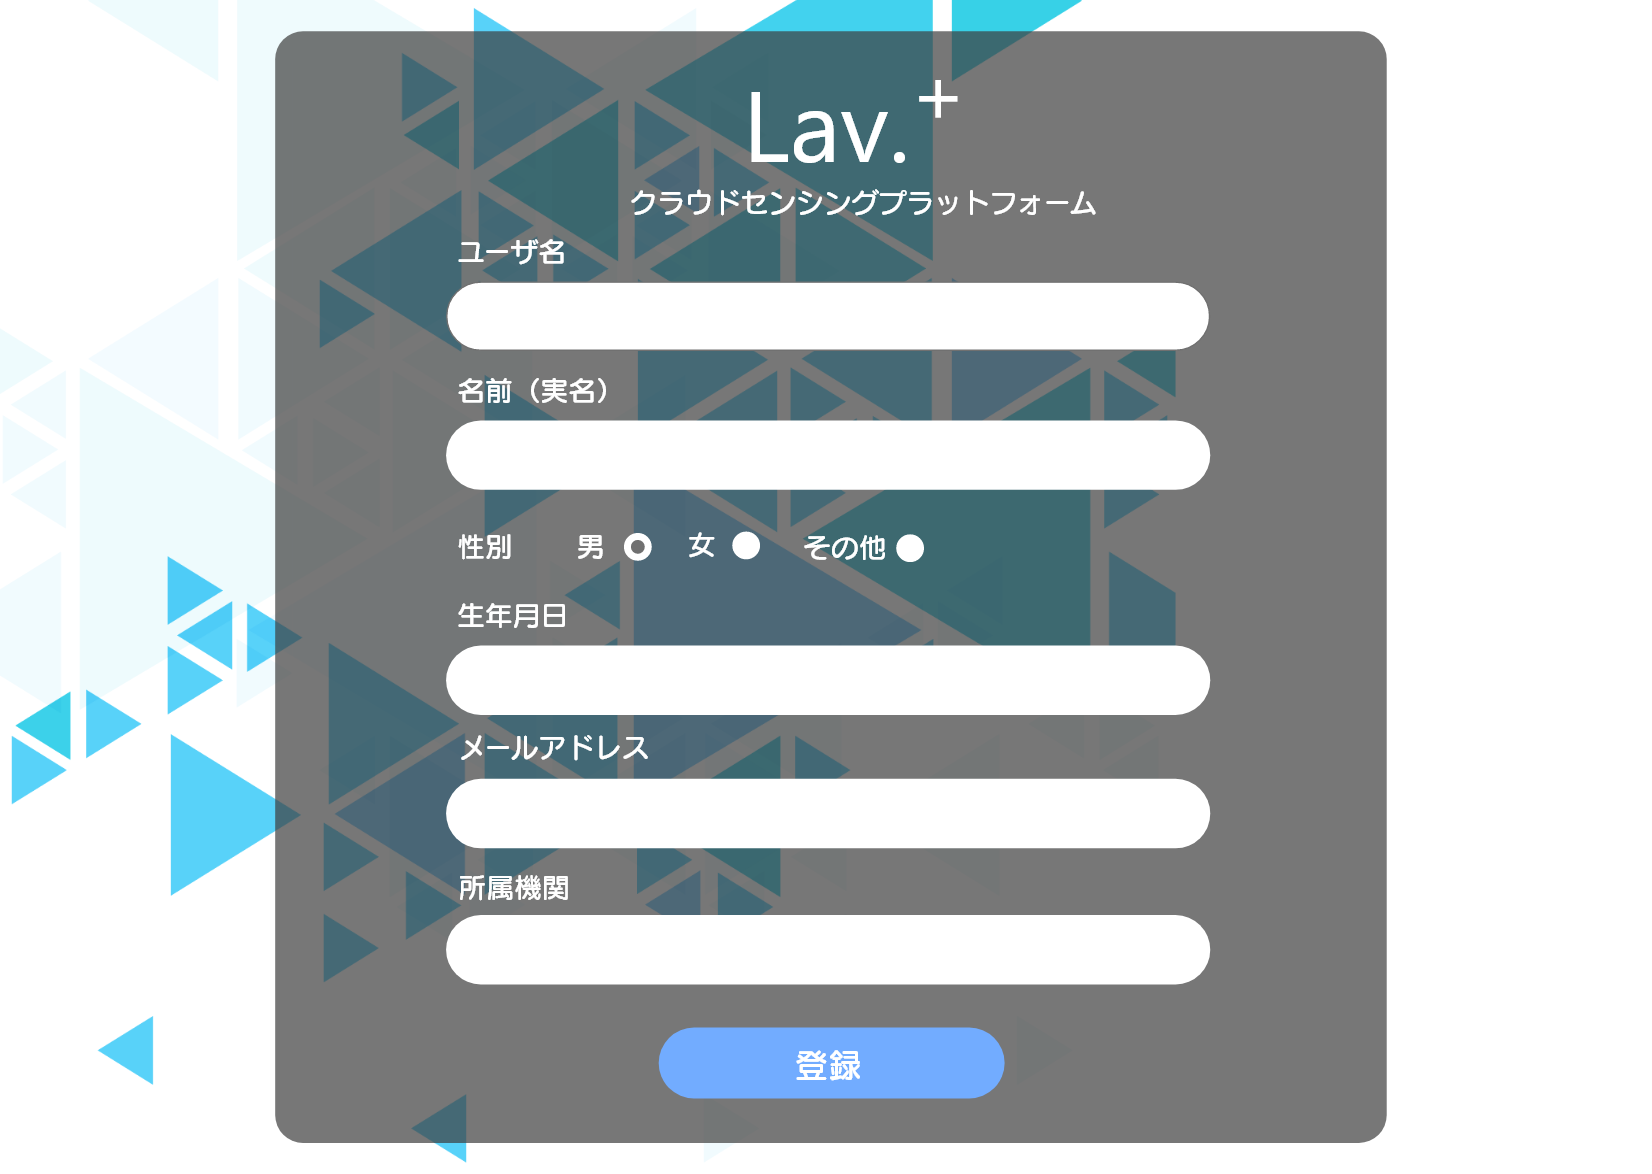
\includegraphics[width=120mm]{Signup.png}
  \caption{ユーザ登録画面}
  \label{baseSetting}
\end{figure}

Webアプリでは,まず依頼者がユーザ登録を行う.
ユーザ登録では,サーバのUserモデルに合わせたフォームを作成し要求仕様の3.2.3項「ラヴラスの利用及び利用規約の方針」に基づき本名,性別,生年月日,eメールアドレス,所属機関の5項目を必須項目とする.
入力が完了し送信ボタンのタップにより,サーバの「/singup」エンドポイントに入力情報が送信され登録完了となる.
次に,新規センシングプロジェクトを作成する.
センシングプロジェクトの入力フォームは入力項目が多いため,要求仕様の3.2.4項「利用者への配慮」のユーザインターフェイスの配慮に対応し,「基本設定」「概要と目的」「有効期限」「センサ設定」「時空間フェンシング設定」の項目の5ページに分け,さらに入力の複雑な項目に対して入力操作を簡易化する仕組みで入力操作の向上を図っている.
各ページの右上に前のページに戻るボタン,入力フォームの下部に次の入力項目に遷移するためのボタンを設置する.
これらのページは,遷移を行っても内部的に入力されたフォームの情報を保持しており,入力を前のページに戻り修正が可能である.
% (img baseStting.png cap: 基本設定ページの入力画面と入力例)
\begin{figure}[H]
  \centering
  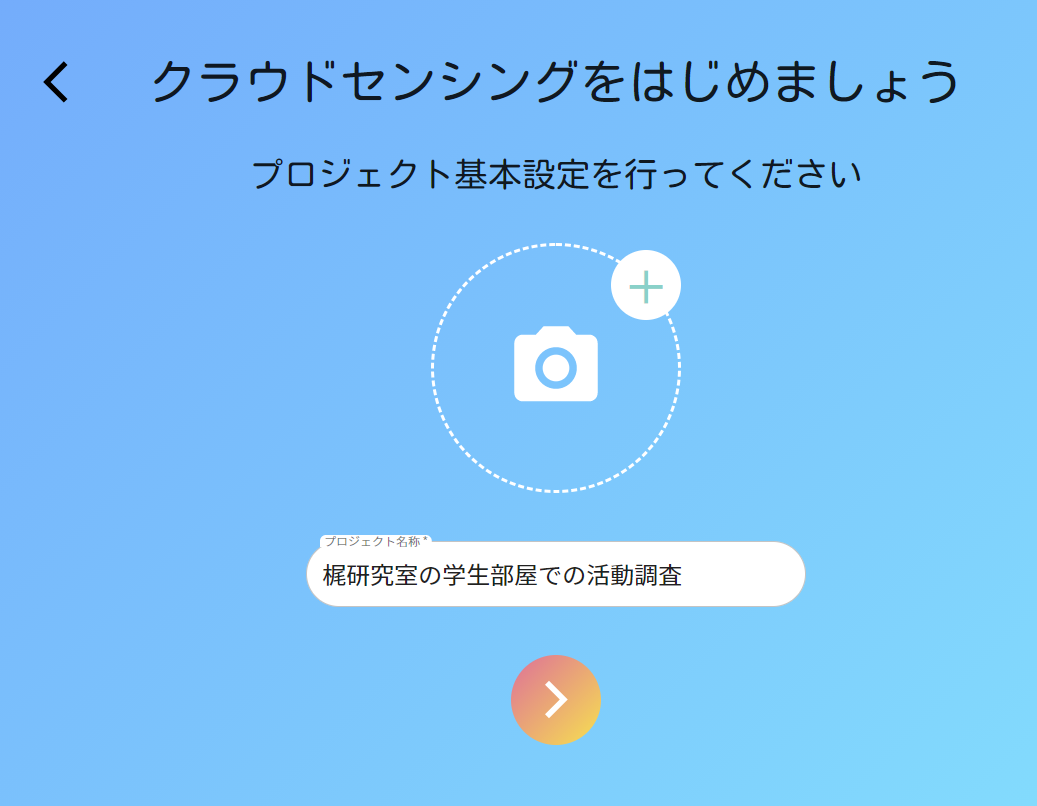
\includegraphics[width=80mm]{baseSetting.png}
  \caption{基本設定ページの入力画面と入力例}
  \label{baseSetting}
\end{figure}

基本設定ページ(図\ref{baseSetting})では,サムネイル用画像とセンシングプロジェクトの名称の入力を行う.
この入力ページでは,プロジェクトの名称のみが必須項目であるため,サムネイル用画像は任意とする.
この2つの項目は,サーバに定義されたProjectモデルの「title」と「image」に対応している.
% (img overview.png cap: 概要と目的ページの入力画面と入力例)
\begin{figure}[H]
  \centering
  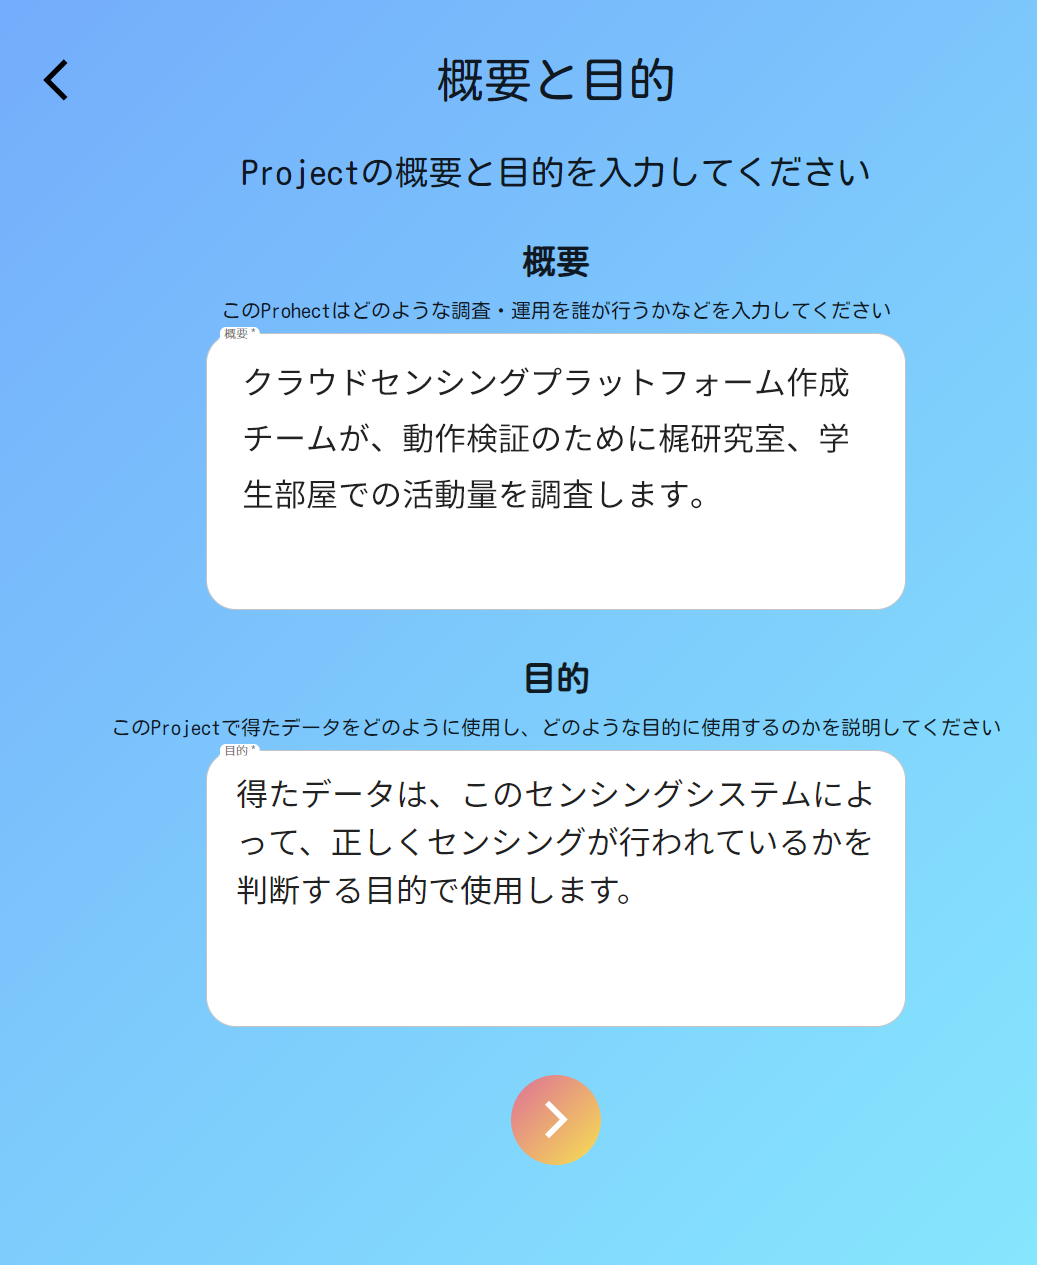
\includegraphics[width=80mm]{overview.png}
  \caption{概要と目的ページの入力画面と入力例}
  \label{overview}
\end{figure}

概要と目的ページ(図\ref{overview})では,概要と目的の入力を行う.
この入力ページでは,どちらの入力項目も必須項目であり,最低文字数20文字以上の入力が必要となっている.
この2つの項目は,サーバに定義されたProjectモデルの「overview」と「purpose」に対応している.
% (img period.png cap: 有効期限ページの入力画面と入力例)
\begin{figure}[H]
  \centering
  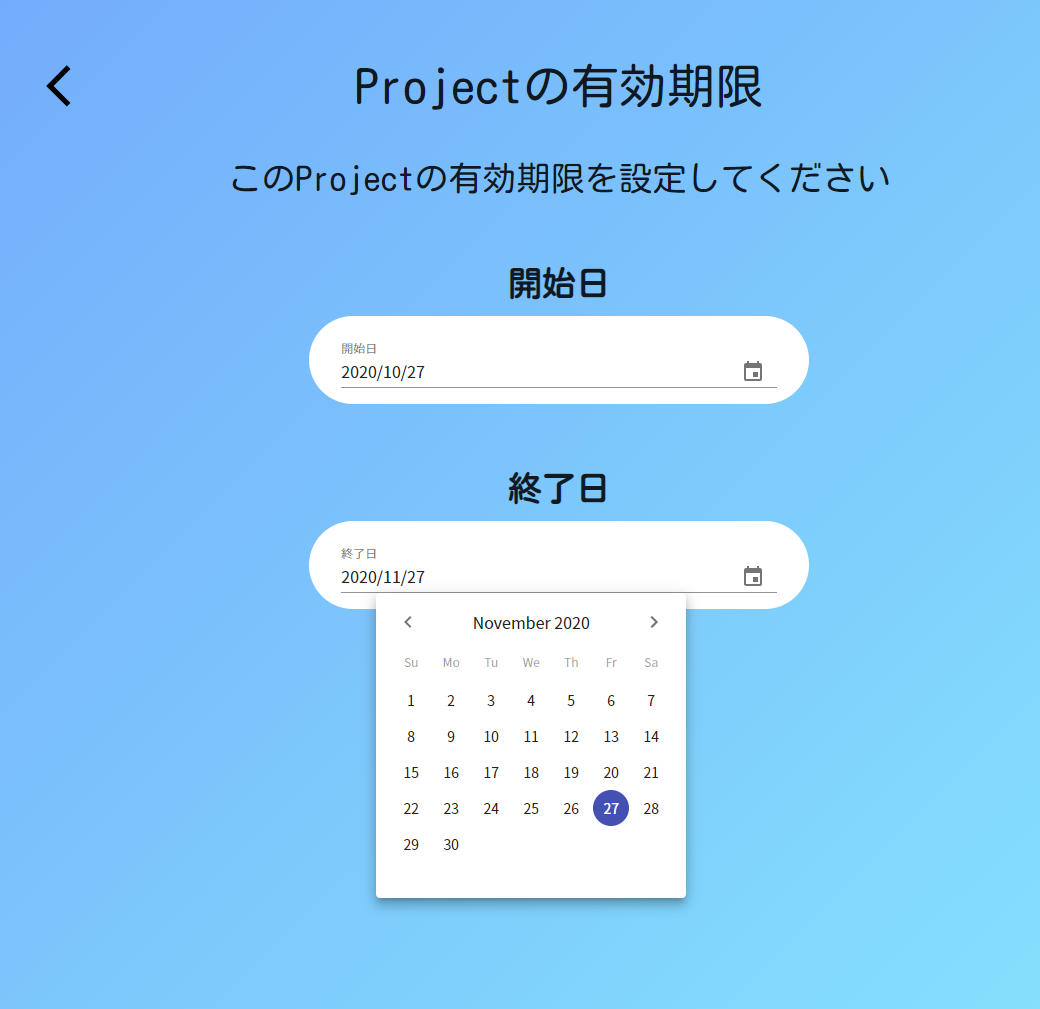
\includegraphics[width=100mm]{period.png}
  \caption{有効期限ページの入力画面と入力例}
  \label{period}
\end{figure}

有効期限ページ(図\ref{period})では,センシング開始日とセンシング終了日入力を行う.
この入力ページでは,どちらの入力項目も必須項目である.
入力フォームは,日付の入力を簡易化するためにカレンダーのポップアップからの入力を可能にする.
この2つの項目は,サーバに定義されたProjectモデルの「startDate」と「endDate」に対応している.
% (img sensors.png cap: センサ設定ページの入力画面と入力例)
\begin{figure}[H]
  \centering
  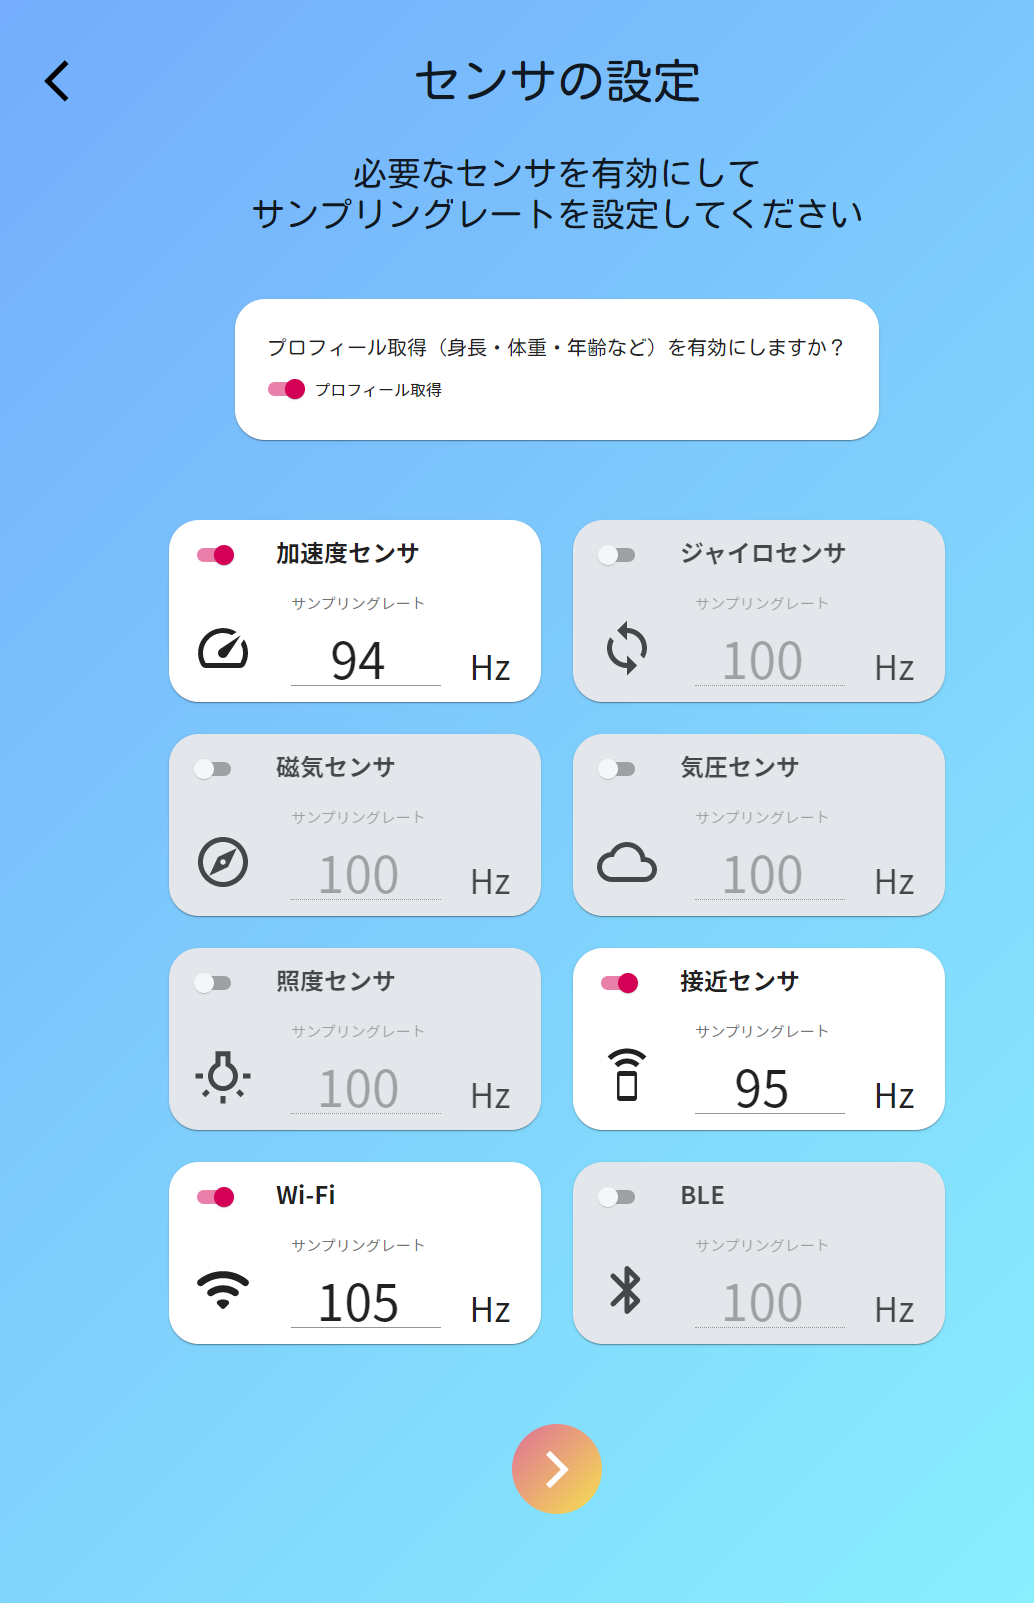
\includegraphics[width=100mm]{sensors.png}
  \caption{センサ設定ページの入力画面と入力例}
  \label{sensors}
\end{figure}

センサ設定ページ(図\ref{sensors})では,協力者に自身の基礎情報を求めるかの有無とセンサの設定を行う.
協力者に協力者の基礎情報を求める設定は,3.3.2項「センシングデータの管理や各プロジェクトを管理するサーバの実装」にも記述があるが,現在実装には至っていないため定義のみとなる.
この入力ページでは,一つ以上のセンサの設定が必須である.
このページのフォームの入力方法はトグルスイッチを採用しており,トグルスイッチにより有効になった設定と無効な設定を判別しやすいようにそれぞれの項目が明るくなるようになっている.
また,各センサの設定は文字だけでなくアイコンを用いてそれぞれのセンサの設定を視覚的に判別しやすいようにしており,トグルスイッチによりサンプリングレートの入力が有効化されサンプリングレートの設定を行う.
この2つの項目は,サーバに定義されたSensingSettingモデルの「isProvidedProfile」と「sensors」に対応している.
% (img areaInput.png cap: 時空間フェンシング設定ページのエリア入力画面と入力例)
\begin{figure}[H]
  \centering
  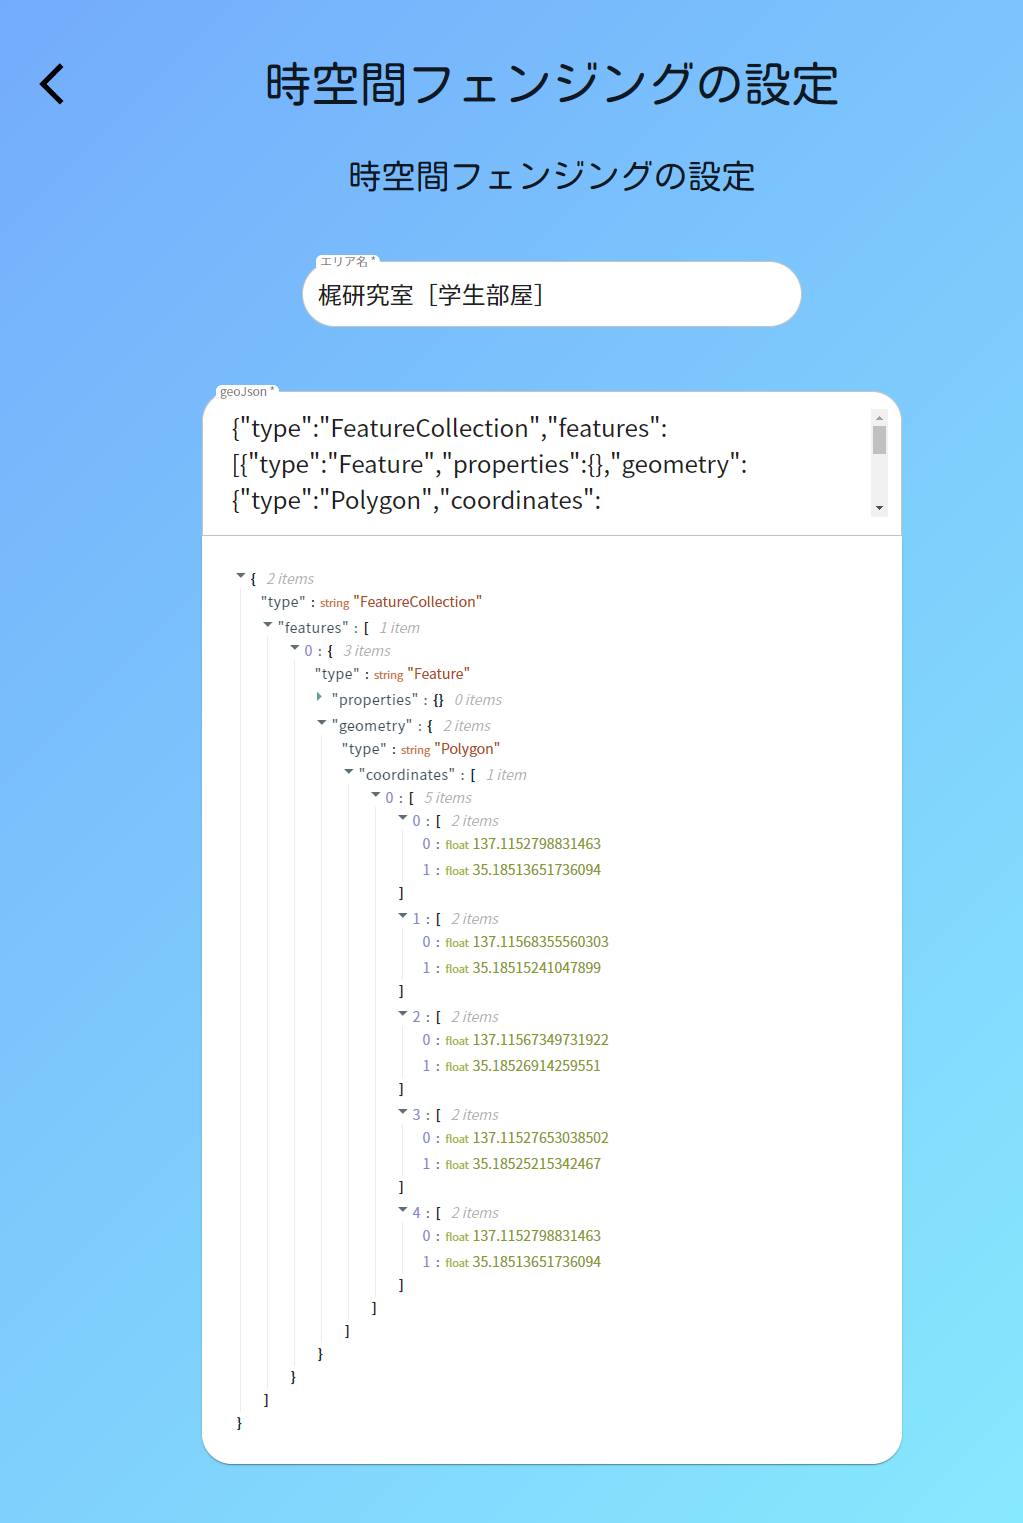
\includegraphics[width=120mm]{areaInput.png}
  \caption{時空間フェンシング設定ページのエリア入力画面と入力例}
  \label{areaInput}
\end{figure}

時空間フェンシング設定ページ(図\ref{areaInput})では,時空間フェンシングに必要なエリアの設定と時間帯の設定を行う.
この入力ページでは,エリア名の入力とエリア設定,時間帯を1つ以上の設定が必須である.
エリアの入力では,GeoJSON形式のテキストの入力を行う.
この入力フォームは,geojson.io\cite{geojson}等のサイトを用いてGeoJSON形式のテキストを取得・入力を前提としている.
図\ref{geojsonIo}は,geojson.ioを利用してGeoJSON形式のテキストを取得する例である.
% (img geojsonIo.png cap: geojson.ioを利用したGeoJSON形式のテキストの取得と入力例)
\begin{figure}[H]
  \centering
  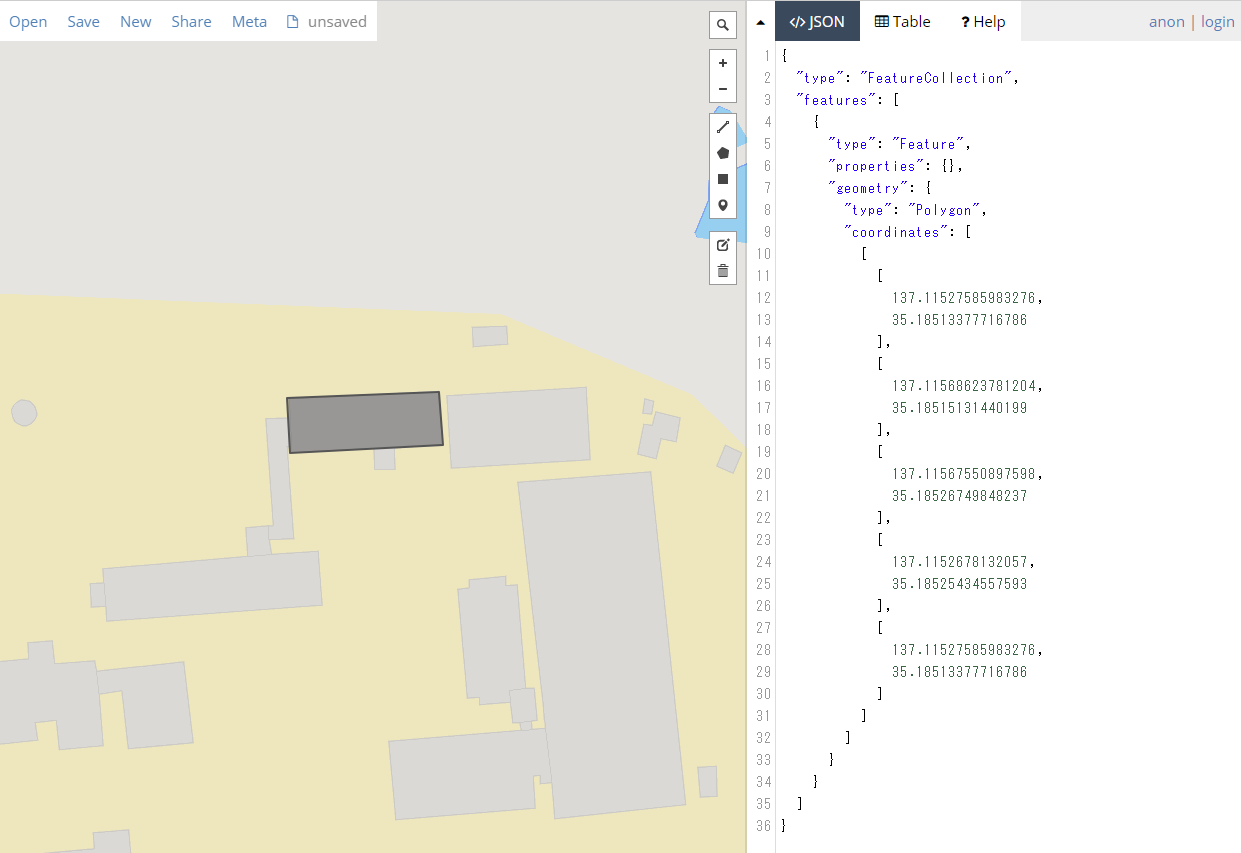
\includegraphics[width=150mm]{geojsonIo.png}
  \caption{geojson.ioを利用したGeoJSON形式のテキストの取得と入力例}
  \label{geojsonIo}
\end{figure}

% (img geojsonIo.png cap: エリア設定入力にGeoJSONでない形式のテキストを入力する例)
\begin{figure}[H]
  \centering
  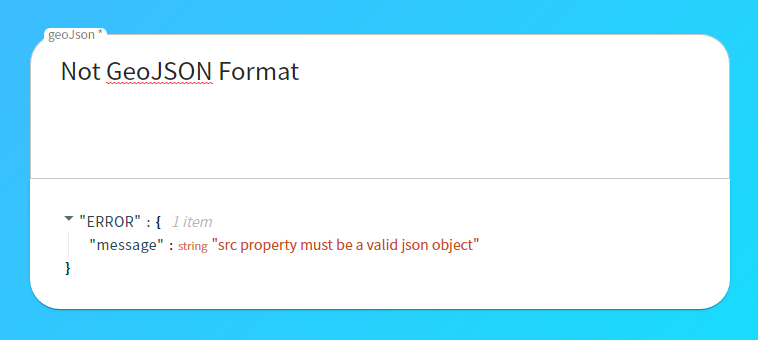
\includegraphics[width=120mm]{notGeoJSONFormat.png}
  \caption{エリア設定入力にGeoJSONでない形式のテキストを入力する例}
  \label{fig401}
\end{figure}

取得したGeoJSON形式のテキストを入力すると,入力フォームの下部に整形されたGeoJSONの情報の確認が可能である.
図\ref{fig401}のようにGeoJSON形式でない文字を入力すると,エラーが表示される様になっているため,入力が正常に行われているのかの確認が可能である.

% (img timeInput.png cap: 時空間フェンシング設定ページの時間帯入力画面と入力例)
\begin{figure}[H]
  \centering
  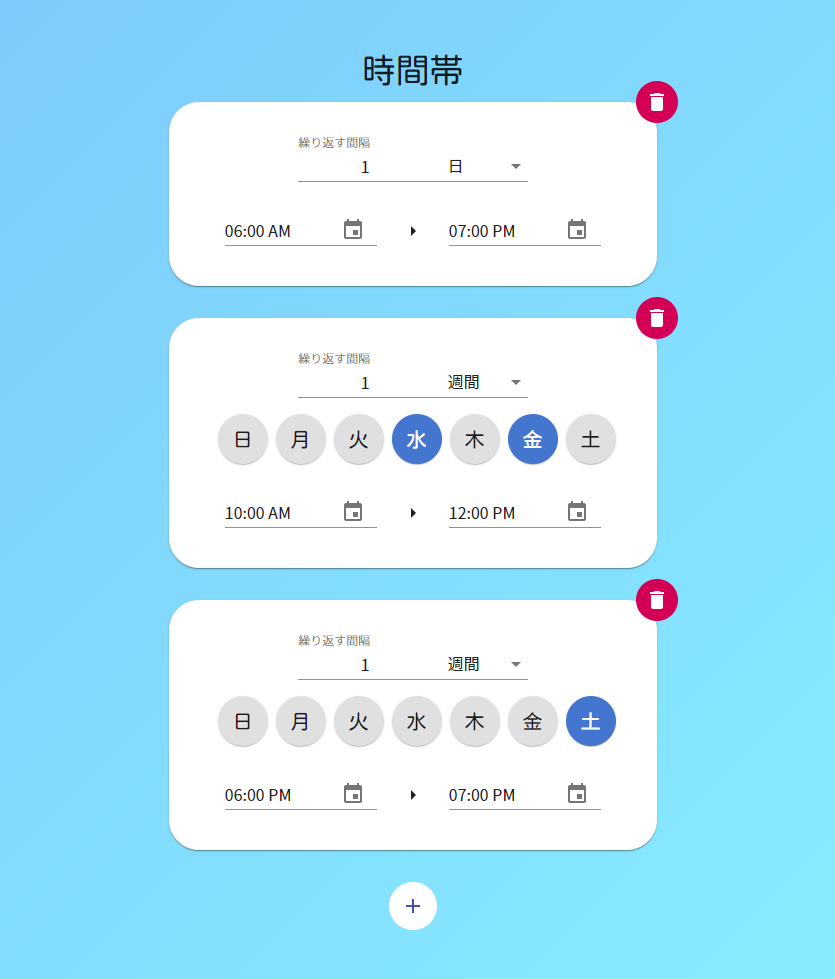
\includegraphics[width=120mm]{timeInput.png}
  \caption{時空間フェンシング設定ページの時間帯入力画面と入力例}
  \label{timeInput}
\end{figure}

% (img timeModal.png cap: 時間の入力モーダル)

\begin{figure}[H]
  \centering
  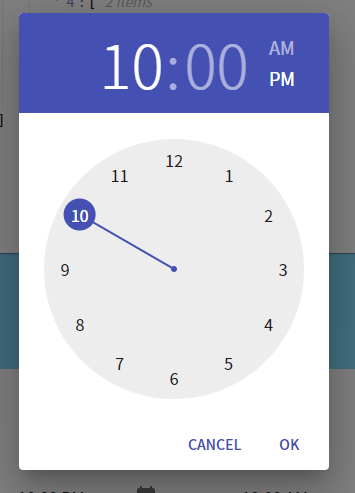
\includegraphics[width=50mm]{timeModal.png}
  \caption{時間の入力モーダル}
  \label{timeModal}
\end{figure}

時間帯の入力フォームでは,3.3.2項「センシングデータの管理や各プロジェクトを管理するサーバの実装」で定義した複数の時間帯を定義可能なフォーマットに対応した入力フォームを作成する.
このフォームは,繰り返す間隔の数字入力とその右側に単位の選択を行うセレクタがあり,セレクタでは「日」と「週間」のどちらかを選択する.
セレクタで「週間」を選択した場合のみ,その下部に曜日を示すボタンが表示され,ボタンをクリックし曜日の指定を行う.
最下部には開始時間と終了時間の入力項目があり,それぞれのフォームのクリックにより,図\ref{timeModal}のような時間を入力するモーダルが表示され時間の入力を行う.
複数の時間帯を定義する場合は,フォーム下部の+ボタンをクリックにより複数の時間帯を定義できる.
また,定義した時間帯の削除を行う場合はフォーム右上のゴミ箱のアイコンをクリックする.
この3つの項目は,サーバに定義されたSensingSettingモデルの「areaName」と「geo」と「periodOftimes」に対応している.
以上の項目をすべて入力後の送信ボタンクリックにより,サーバの「/project」及び「/sensing-setting」エンドポイントに入力情報が送信される.
センシングプロジェクトの定義が完了となり開始日になると,センシングプロジェクトが開始される.

\begin{figure}[H]
  \centering
  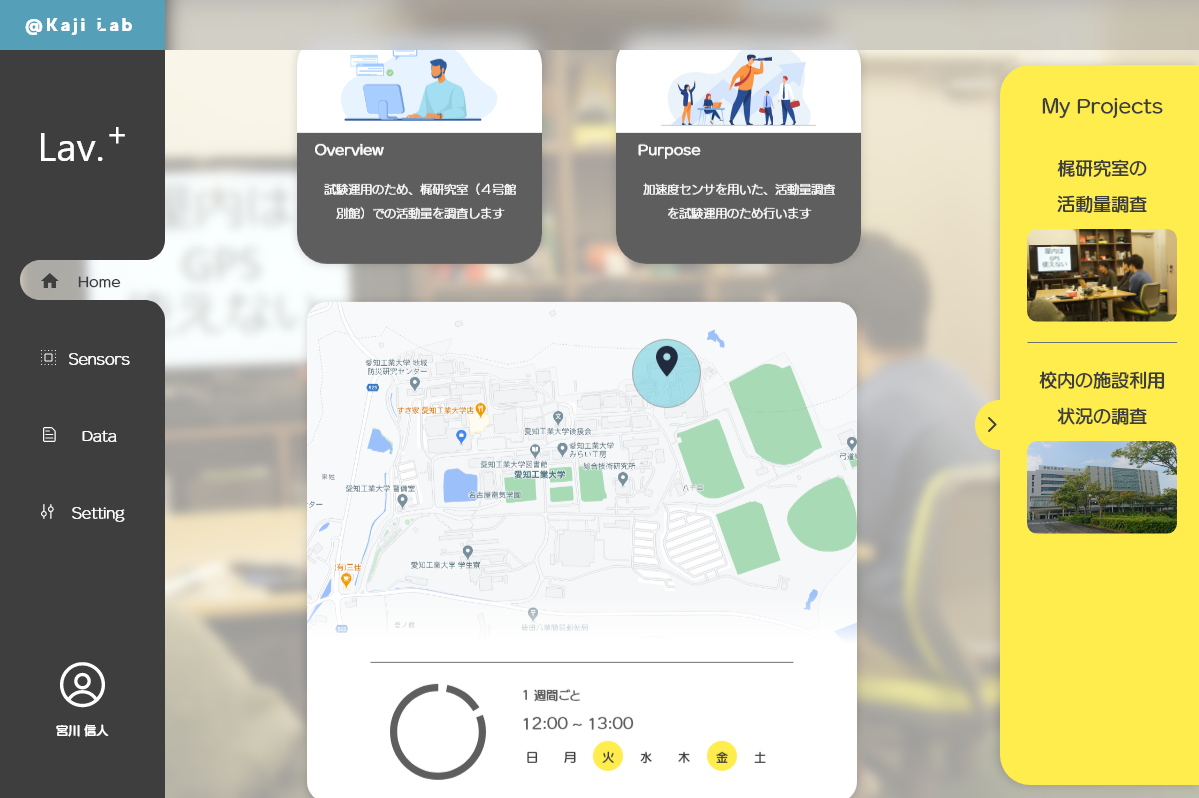
\includegraphics[width= 150mm]{Dashboard.png}
  \caption{管理画面ページ}
  \label{server}
\end{figure}

センシングプロジェクトの定義を終了すると,管理画面にて定義したセンシングプロジェクトの情報閲覧が可能となる.
協力者からセンシングデータを提供されると,その管理画面よりそのセンシングデータのダウンロードが可能となる.
ラヴラスでは依頼者1人による複数のプロジェクトの作成を想定し,管理画面の右側に表示されたメニューより作成したセンシングプロジェクトの切り替え及び追加作成が可能となっている.

\begin{figure}[H]
  \centering
  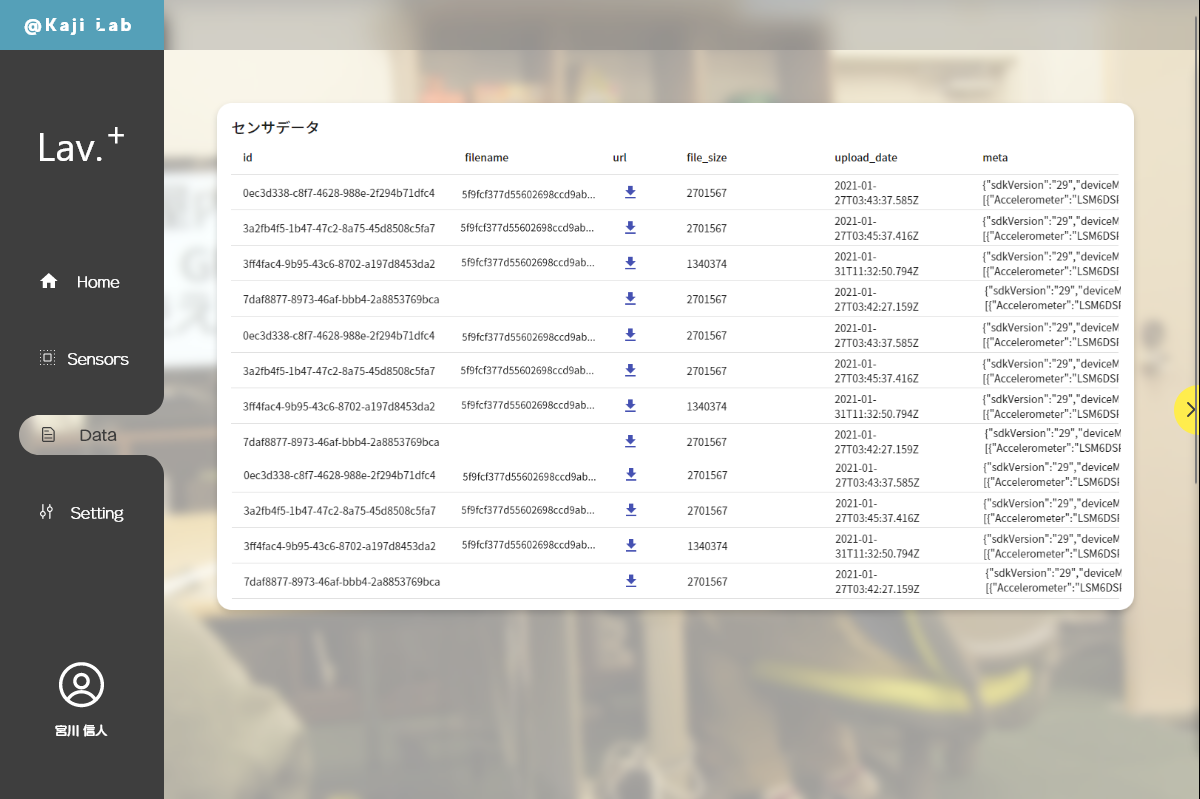
\includegraphics[width= 150mm]{Dashboard-SensingData.png}
  \caption{提供されたセンシングデータの一覧及びダウンロードを行うページ}
  \label{server}
\end{figure}

提供されたセンシングデータのダウンロードは,Dataメニューのクリックによりセンシングデータの一覧が表示され,ファイル名,ファイルサイズ,アップロード日,メタデータの情報を確認できる.
センシングデータのダウンロードは,一覧の各列のダウンロードボタンのクリックにより可能である.
% -----------------------------------------------

\subsection{協力者用のセンシングスマホアプリの実装}

\begin{figure}[H]
  \centering
  \includegraphics[width= 150mm]{serverApp.png}
  \caption{サーバとスマホアプリの連携}
  \label{server}
\end{figure}


ラヴラスでは,協力者がセンシングプロジェクト毎にスマホアプリをインストールする手間を省くため,協力者専用のAndroidアプリケーションを作成する.
第1章でも述べたように,スマートフォンの利用者は使用頻度の低いアプリケーションを削除する傾向にある.
理由としては,ストレージの容量確保のためであったり,整理整頓であったりと様々である.
例えば,本プラットフォームのような基盤を用いず,個別の専用アプリケーションを作成し,クラウドセンシングを行うとする.
この場合,専用アプリケーションの数は研究の数と比例する.
クラウドセンシングを利用して行いたい人が増えれば増えるほど,個別の専用アプリケーションも増えていく.
その都度協力者はアプリケーションをインストールする必要がある.
インストールには時間や手間がかかり,ストレージを使用してしまう.
1回ならまだしも,インストールの回数が2回3回と増えていくと,クラウドセンシング自体が面倒になり,非協力的になってしまう可能性がある.
ストレージの使用容量が微量だったとしても,空き容量がなくなった場合に真っ先に削除される可能性もある.
依頼者が別のクラウドセンシングを行う際,前回のシステムをそのまま使うとしても,アップデートや再インストールが必要となるため,協力者にとっては負担になる.
また,一定期間クラウドセンシングを行わなかった場合,協力者は「もうこのアプリケーションでのセンシングは終わったのだ」と解釈し,削除する可能性がある.
こうなると,いざもう一度センシングを行おうとなったときに協力者がいるとは限らない.
個別でクラウドセンシングアプリケーションを作成する問題点として,仕様や操作法の違いも挙げられる.
クラウドセンシングは一定の基準が定められている訳ではないため,依頼者独自の仕様や操作法である.
アプリ毎に仕様を理解し操作するのは協力者にとって大きな負担になる.
依頼者が所属している研究室の教授であったり,友人である場合,そのような負担も気にならないかもしれないが,赤の他人であった場合,
協力者が本スマホアプリをインストールすれば,本プラットフォームで作成されたセンシングプロジェクトに協力が可能となる.
これにより,依頼者はクラウドセンシングを利用するために,一からセンシング専用のスマホアプリを開発する必要がなくなり,協力者はクラウドセンシングに協力するために,何度もインストールする必要がなくなる.

本スマホアプリはサーバと連携し,センシングプロジェクトの受信やセンシングデータファイルとメタデータのアップロードを行う.
センシングプロジェクトは適宜サーバから取得し,本スマホアプリ内のデータベースに登録する.
新規のセンシングプロジェクトの場合は新しく登録し,既存のセンシングプロジェクトの場合は内容が変更している可能性を考慮して最新の方に更新する.
データベースより現在時刻から一番近い指定開始時間を検索し,指定開始時間と指定終了時間を時空間フェンシングに設定する.
また,設定した時間と同じセンシングプロジェクトのエリアとプロジェクトIDも設定しておく.
プロジェクトIDは時空間内に進入した際に送られる通知画面に表示されるプロジェクト内容の検索に用いる.

時空間フェンシングは位置情報取得を最小限にするために,まず時間判定を行い,センシングプロジェクトで指定された開始時間にエリア判定を行う.
時間判定とエリア判定を平行して行った場合でも,問題なく時空間フェンシングは動作する.
しかし,我々のクラウドセンシングの中枢として,協力者の負担軽減がある.
位置情報の収集とスマートフォンの電池の消耗は直接的な関係がある.
例えば,位置情報データの精度が高ければ高いほど電池の消耗は激しくなる.
また,位置情報の計算頻度が高ければ高いほど電池の消費量は増加する.
つまり,位置情報の精度と計算頻度が高いほど,より多くの電池量を消費するのである.
そのため,スマートフォンの負担を軽減するには,低い精度と計算頻度で妥協する必要がある.
しかし,時空間フェンシングを行う上で,位置情報は非常に重要な情報である.
位置情報の精度が低いと,実際にはエリア内に進入しているのにスマートフォン上ではエリア外となってしまったり,反対にエリア外にいるのにエリア内に進入しているとなってしまう可能性がある.
それにより,途中でセンシングが終了してしまったり,ずっとエリア内にいるのにセンシング依頼通知が送られてないなどセンシングに支障をきたしてしまう.
よって,位置情報の精度の低減もできない.
指定開始時間以前に指定エリア内に入っていてもセンシングは開始しないし,スマートフォンの充電を無駄に消耗させてしまう.
そのため,指定開始時間後にエリア判定を行う.

協力者が指定センシングエリア内に進入したか否かは,点の多角形に対する内外判定\cite{naigai}で判定する.
点の多角形に対する内外判定を図\ref{naigaihantei}に示す.
点の内外判定とは,まず点(赤丸)から多角形に対して水平線を引く.
その線と多角形との交点(青丸)の数が奇数個であれば多角形よりも内側にいる,偶数個であれば多角形よりも外側にいると判定できる.
この場合,丁度線と多角形の辺が重なったり,線と多角形の頂点と重なると,誤った判定を行ってしまう.
しかし,緯度経度は小数点以下が7桁もあり,位置情報は変化し続けるため,丁度重なる場合は今回考えないものとしている.
実装当初は内外判定ではなく条件分岐を用いて,エリア判定を行っていた.
現在位置の緯度が指定エリアの最北端よりも低く最南端よりも高い,また経度が指定エリアの最東端よりも低く最西端よりも高い場合,指定エリア内にいると判定した.
しかし,この条件分岐を用いると,自ずと判定範囲が矩形になってしまう.
そうなった場合,正常にエリア判定できるのは緯度経度と平行な矩形のみとなる.
例えば,指定センシングエリアがひし形の場合を想定する.
正常なエリア判定としては,図\ref{risou}の通り現在地(赤丸)にいた場合はエリア内に進入していないため,通知は送られないはずである.
しかし,条件分岐を用いたエリア判定の場合は,ひし形の外側にひし形の頂点を辺の中心とした矩形の判定エリアが形成されるため,図\ref{bunki}のように現在地がエリア内にいると判定され,誤って通知が送られてしまう.
一方で,点の内外判定は現在地から水平に引いた線とひし形のエリアの交点(青丸)が2つと偶数個であるため,エリア外と判定できる(図\ref{orr}).
これにより,依頼者が図\ref{naigaihantei}のようにどれだけ複雑な多角形のエリアを設定しても,内部か否かは判定可能である.
今回は実装は行っていないが円のようなエリアでも判定は可能である.
また,今回はGPSのみを用いたエリア判定のため,平面的なエリア判定しか行えない.
1階や2階などの立体的なエリア判定は今後の課題とする.

\begin{figure}[H]
    \begin{center}
      \begin{tabular}{c}
  
        % 1
        \begin{minipage}{0.5\hsize}
            \begin{center}
            
            \begin{tikzpicture}
   
                
                \coordinate  (A) at (1,1); %点A
                \coordinate  (B) at (5,1); %点B
                \coordinate  (C) at (4,2); %点C
                \coordinate  (D) at (4,4); %点D
                \coordinate  (E) at (1,4); %点D
                \coordinate  (F) at (1,2); %点D
                \coordinate  (J) at (2,2); %点D
                \coordinate  (K) at (2,3); %点D
                \coordinate  (G) at (3,3); %点D
                \coordinate  (H) at (3,2); %点D
                \coordinate  (I) at (3,1.5); %点D
                \coordinate  (L) at (1.5,2.5); %点D
                \coordinate  (M) at (4.5,1.5); %点D
                \coordinate  (N) at (2,2.5); %点D
                \coordinate  (O) at (3,2.5); %点D
                \coordinate  (P) at (4,2.5); %点D
                % \coordinate [label=現在地](E) at (0.5,1.5); %点E
                \foreach \P in {A,B,C,D,E,F,G,J,K,H} \fill[black] (\P) circle (0.08);  %点A,B,Cに黒丸
                
                \foreach \P in {I,L} \fill[red] (\P) circle (0.08);
                \draw (A) -- (B) -- (C) -- (D) -- (E) -- (F) -- (J) -- (K)-- (G) -- (H) -- cycle;
                % \draw (0,0) -- (3,0) -- (0,1) -- cycle;
                % \draw (3,0) -- (6,0) -- (6,1) -- cycle;
                % \draw (6,1) -- (6,2) -- (3,2) -- cycle;
                % % \draw (0,1) -- (0,2) -- (3,2) -- cycle;
                % \fill[lightgray] (A) -- (B) -- (C) -- (D) -- cycle;
                \draw[->,>=stealth,semithick] (3,1.5)--(7,1.5)node[above]{$交点1つ$};
                \draw[->,>=stealth,semithick] (1.5,2.5)--(7,2.5)node[above]{$交点3つ$};
                \foreach \P in {M,N,O,P} \fill[cyan] (\P) circle (0.08);
        
            \end{tikzpicture}
            \hspace{1.9cm} 点が多角形より内側の場合は交点が奇数個


        \end{center}
        \end{minipage}

        % 1
        \begin{minipage}{0.5\hsize}
            \begin{center}
            
            \begin{tikzpicture}
   
                
                \coordinate  (A) at (1,1); %点A
                \coordinate  (B) at (5,1); %点B
                \coordinate  (C) at (4,2); %点C
                \coordinate  (D) at (4,4); %点D
                \coordinate  (E) at (1,4); %点D
                \coordinate  (F) at (1,2); %点D
                \coordinate  (J) at (2,2); %点D
                \coordinate  (K) at (2,3); %点D
                \coordinate  (G) at (3,3); %点D
                \coordinate  (H) at (3,2); %点D
                \coordinate  (I) at (1,1.5); %点D
                \coordinate  (L) at (2.5,2.5); %点D
                \coordinate  (M) at (4.5,1.5); %点D
                \coordinate  (N) at (2,1.5); %点D
                \coordinate  (O) at (3,2.5); %点D
                \coordinate  (P) at (4,2.5); %点D
                % \coordinate [label=現在地](E) at (0.5,1.5); %点E
                \foreach \P in {A,B,C,D,E,F,G,J,K,H} \fill[black] (\P) circle (0.08);  %点A,B,Cに黒丸
                
                \foreach \P in {I,L} \fill[red] (\P) circle (0.08);
                \draw (A) -- (B) -- (C) -- (D) -- (E) -- (F) -- (J) -- (K)-- (G) -- (H) -- cycle;
                % \draw (0,0) -- (3,0) -- (0,1) -- cycle;
                % \draw (3,0) -- (6,0) -- (6,1) -- cycle;
                % \draw (6,1) -- (6,2) -- (3,2) -- cycle;
                % % \draw (0,1) -- (0,2) -- (3,2) -- cycle;
                % \fill[lightgray] (A) -- (B) -- (C) -- (D) -- cycle;
                \draw[->,>=stealth,semithick] (1,1.5)--(6.5,1.5)node[above]{$交点2つ$};
                \draw[->,>=stealth,semithick] (2.5,2.5)--(7,2.5)node[above]{$交点2つ$};
               \foreach \P in {M,N,O,P} \fill[cyan] (\P) circle (0.08);
               
            \end{tikzpicture}
            \hspace{1.6cm} 点が多角形より外側の場合は交点が偶数個
        \end{center}
        \end{minipage}
  
        
  
      \end{tabular}
      
      
      \caption{点の多角形に対する内外判定}
      \label{naigaihantei}
    \end{center}
  \end{figure}

\begin{figure}[H]
    \begin{center}
      \begin{tabular}{c}
  
        % 1
        \begin{minipage}{0.5\hsize}
            \begin{center}
            
            \begin{tikzpicture}
   
                \draw[->,>=stealth,semithick] (-0.1,0)--(6.5,0)node[above]{$lng$}; %x軸
                \draw[->,>=stealth,semithick] (0,-0.1)--(0,2.5)node[right]{$lat$}; %y軸
                \draw (0,0); %原点
 
                \coordinate  (A) at (0,1); %点A
                \coordinate  (B) at (3,0); %点B
                \coordinate  (C) at (6,1); %点C
                \coordinate  (D) at (3,2); %点D
                \coordinate [label=現在地](E) at (0.5,1.5); %点E
                \foreach \P in {A,B,C,D} \fill[black] (\P) circle (0.08);  %点A,B,Cに黒丸
                \foreach \P in {E} \fill[red] (\P) circle (0.08);
                 \draw (A) -- (B) -- (C) -- (D) -- cycle;
                % \draw (0,0) -- (3,0) -- (0,1) -- cycle;
                % \draw (3,0) -- (6,0) -- (6,1) -- cycle;
                % \draw (6,1) -- (6,2) -- (3,2) -- cycle;
                % \draw (0,1) -- (0,2) -- (3,2) -- cycle;
                \fill[lightgray] (A) -- (B) -- (C) -- (D) -- cycle;

        
            \end{tikzpicture}
            \hspace{1.6cm} 現在地→エリア外\\エリア判定上→エリア外
            \caption{正常なエリア判定}
            \label{risou}
        \end{center}
        \end{minipage}
  
        % 2
        \begin{minipage}{0.5\hsize}
          \begin{center}
            \begin{tikzpicture}
   
                \draw[->,>=stealth,semithick] (-0.1,0)--(6.5,0)node[above]{$lng$}; %x軸
                \draw[->,>=stealth,semithick] (0,-0.1)--(0,2.5)node[right]{$lat$}; %y軸
                \draw (0,0); %原点
                \coordinate (A) at (0,1); %点A
                \coordinate (B) at (3,0); %点B
                \coordinate (C) at (6,1); %点C
                \coordinate (D) at (3,2); %点D
                \foreach \P in {A,B,C,D} \fill[black] (\P) circle (0.08);  %点A,B,Cに黒丸
                
                \draw (A) -- (B) -- (C) -- (D) -- cycle;
                \draw (0,0) -- (3,0) -- (0,1) -- cycle;
                \draw (3,0) -- (6,0) -- (6,1) -- cycle;
                \draw (6,1) -- (6,2) -- (3,2) -- cycle;
                \draw (0,1) -- (0,2) -- (3,2) -- cycle;
                \fill[lightgray] (0,0) -- (3,0) -- (0,1) -- cycle;
                \fill[lightgray] (3,0) -- (6,0) -- (6,1) -- cycle;
                \fill[lightgray] (6,1) -- (6,2) -- (3,2) -- cycle;
                \fill[lightgray] (0,1) -- (0,2) -- (3,2) -- cycle;
                \fill[lightgray] (A) -- (B) -- (C) -- (D) -- cycle;
                \coordinate [label=現在地](E) at (0.5,1.5); %点E
                \foreach \P in {E} \fill[red] (\P) circle (0.08);
        
            \end{tikzpicture}
            \hspace{1.6cm} 現在地→エリア外\\エリア判定上→エリア内
            \caption{条件分岐による矩形でのエリア判定}
            \label{bunki}
          \end{center}
        \end{minipage}
  
      \end{tabular}
      
      \label{fig:lena}
    \end{center}
  \end{figure}

  \begin{figure}[H]
    \begin{center}
      \begin{tabular}{c}
  
        % 1
        \begin{minipage}{0.5\hsize}
            \begin{center}
            
            \begin{tikzpicture}
   
                \draw[->,>=stealth,semithick] (-0.1,0)--(6.5,0)node[above]{$lng$}; %x軸
                \draw[->,>=stealth,semithick] (0,-0.1)--(0,2.5)node[right]{$lat$}; %y軸
                \draw (0,0); %原点
 
                \coordinate  (A) at (0,1); %点A
                \coordinate  (B) at (3,0); %点B
                \coordinate  (C) at (6,1); %点C
                \coordinate  (D) at (3,2); %点D
                \coordinate  (F) at (1.5,1.5); %点D
                \coordinate  (G) at (4.5,1.5); %点D
                \coordinate [label=現在地](E) at (0.5,1.5); %点E
                \foreach \P in {A,B,C,D,F,G} \fill[black] (\P) circle (0.08);  %点A,B,Cに黒丸
                
                \foreach \P in {E} \fill[red] (\P) circle (0.08);
                 \draw (A) -- (B) -- (C) -- (D) -- cycle;
                % \draw (0,0) -- (3,0) -- (0,1) -- cycle;
                % \draw (3,0) -- (6,0) -- (6,1) -- cycle;
                % \draw (6,1) -- (6,2) -- (3,2) -- cycle;
                % % \draw (0,1) -- (0,2) -- (3,2) -- cycle;
                % \fill[lightgray] (A) -- (B) -- (C) -- (D) -- cycle;
                \draw[->,>=stealth,semithick] (0.5,1.5)--(6.5,1.5);
                \foreach \P in {F,G} \fill[cyan] (\P) circle (0.08);
        
            \end{tikzpicture}
            \hspace{1.6cm} 線とエリアの交点が2つ→エリア外
        \end{center}
        \end{minipage}
  
        
  
      \end{tabular}
      \caption{点の内外判定でのエリア判定}
      \label{orr}
    \end{center}
  \end{figure}

% 本アプリケーションが取得する位置情報は常に正確であるとは限らないため,marginを用いて進入時にはエリアを縮小,退出時には拡大する.

協力者がセンシングプロジェクトで指定された時間帯とエリア内に進入したら,通知を送る.
通知はヘッドアップ通知で,振動ありで送られる.
ヘッドアップ通知により,スマートフォンを使用している際に目に留まりやすく,また振動もあるため,スマートフォンの画面を見ていない時やポケットに入れている時により気がつきやすくなる.
通知のタップにより,アプリケーションを開き,センシング依頼の通知画面が表示される.
通知画面では現在地と指定エリアをGoogle Mapsで,時間帯をバーで,センシングプロジェクトの内容をスクロールで表示し,協力者に確認してもらう.
指定エリアのマップ表示により,テキストよりも指定エリアの広さが解りやすく,現在地との位置関係も把握しやすい.


% センサの処理やセンシングデータファイルの作成などセンシングの大部分は,HASC Loggerという行動センシングデータを収集するアプリケーションの仕組みを参考に実装した.

% サーバとのHTTP通信では,センシングプロジェクトの取得やセンシングデータファイルのアップロードなどを行う.

センシングデータファイルはディレクトリを監視し,ファイルへのセンシングデータ書き込み終了(書き込み用にファイルを開いて閉じた)を判定したとき,協力者のスマートフォンがWi-Fiに接続されていればアップロードされる.
まず協力者が指定エリアから退出した及び指定終了時間になった時,実行中のセンシングを終了する.
センシング終了後,センシングデータを書き込んでいたファイルを閉じた際にイベント判定を行い,ファイルアップロードの段階に入る.
ファイルアップロードでは,まずデータベースにセンシングファイル名とファイルを未アップロードという情報を紐づけて登録する.
次に,Wi-Fiなどのインターネット接続の有無を確認し,接続されている場合のみアップロードを行い,未アップロードの情報を更新する.
携帯回線に接続された状態でセンシングデータをアップロードしてしまうと,協力者のモバイル通信量を使用し負担をかけてしまう.
手動でデータアップロードする場合は,携帯回線を好まない場合にWi-Fiに接続できる場所に移動してからアップロードするなど判断ができるため,アプリケーション側の配慮は必要としない.
しかし,自動でアップロードする場合,判断する余地がないため,負担の少ないWi-Fiに接続時のみにしなければならない.
もし,Wi-Fiに接続されていない場合は,アップロードを見送り,次回ファイルアップロードの段階に入った際にまとめてアップロードする.

協力者の操作を最小限にするため,時空間フェンシングやセンシング,センシングデータのアップロードなどアプリの大部分はバックグラウンドで行う.
そのため,スマホアプリを意識して開く必要はない.
開くのは時空間内に進入した際に送られるヘッドアップ通知をタップした時のみである.
それ以外は基本的に画面上のアイコンをタップしてアプリケーションを開くなどは不要である.
通知画面を承諾した後も,「センシング中はアプリケーションを開いておかなければならない」という仕様ではないため,すぐに閉じても構わない.
アプリケーション自体を終了させなければ,途中でセンシングは終了しない.
バックグラウンドにより,協力者の操作などの負担の軽減に加え,センシングをしているという感覚を意識させないため,より普段の振る舞いをセンシングできる.
% -----------------------------------------------

\section{動作検証}
本センシングプラットフォームを用いて,依頼者側のセンシングプロジェクトの作成やセンシングデータのダウンロード,協力者側の時空間フェンシングや通知,センシングプロジェクトに基づいたセンシング,センシングデータのアップロードなど一連の流れが正常に動作するか検証する.
動作が正常か否かを確認するためにチェック項目を設けた.
依頼者側のチェック項目としては,「センシングプロジェクトを作成できるか」,「アップロードされたセンシングデータはダウンロード可能か」を挙げた.
協力者側のチェック項目としては,「サーバからセンシングプロジェクトを受信できるか」「依頼者によって作成されたセンシングプロジェクトに基づいて,時空間フェンシングができているか」,「指定された時空間内に進入した際にヘッドアップ通知を送っているか」,「正しくセンシングできているか」,「センシング後,Wi-Fi接続時にセンシングデータをアップロードできているか」を挙げた.

\begin{figure}[H]
  \centering
  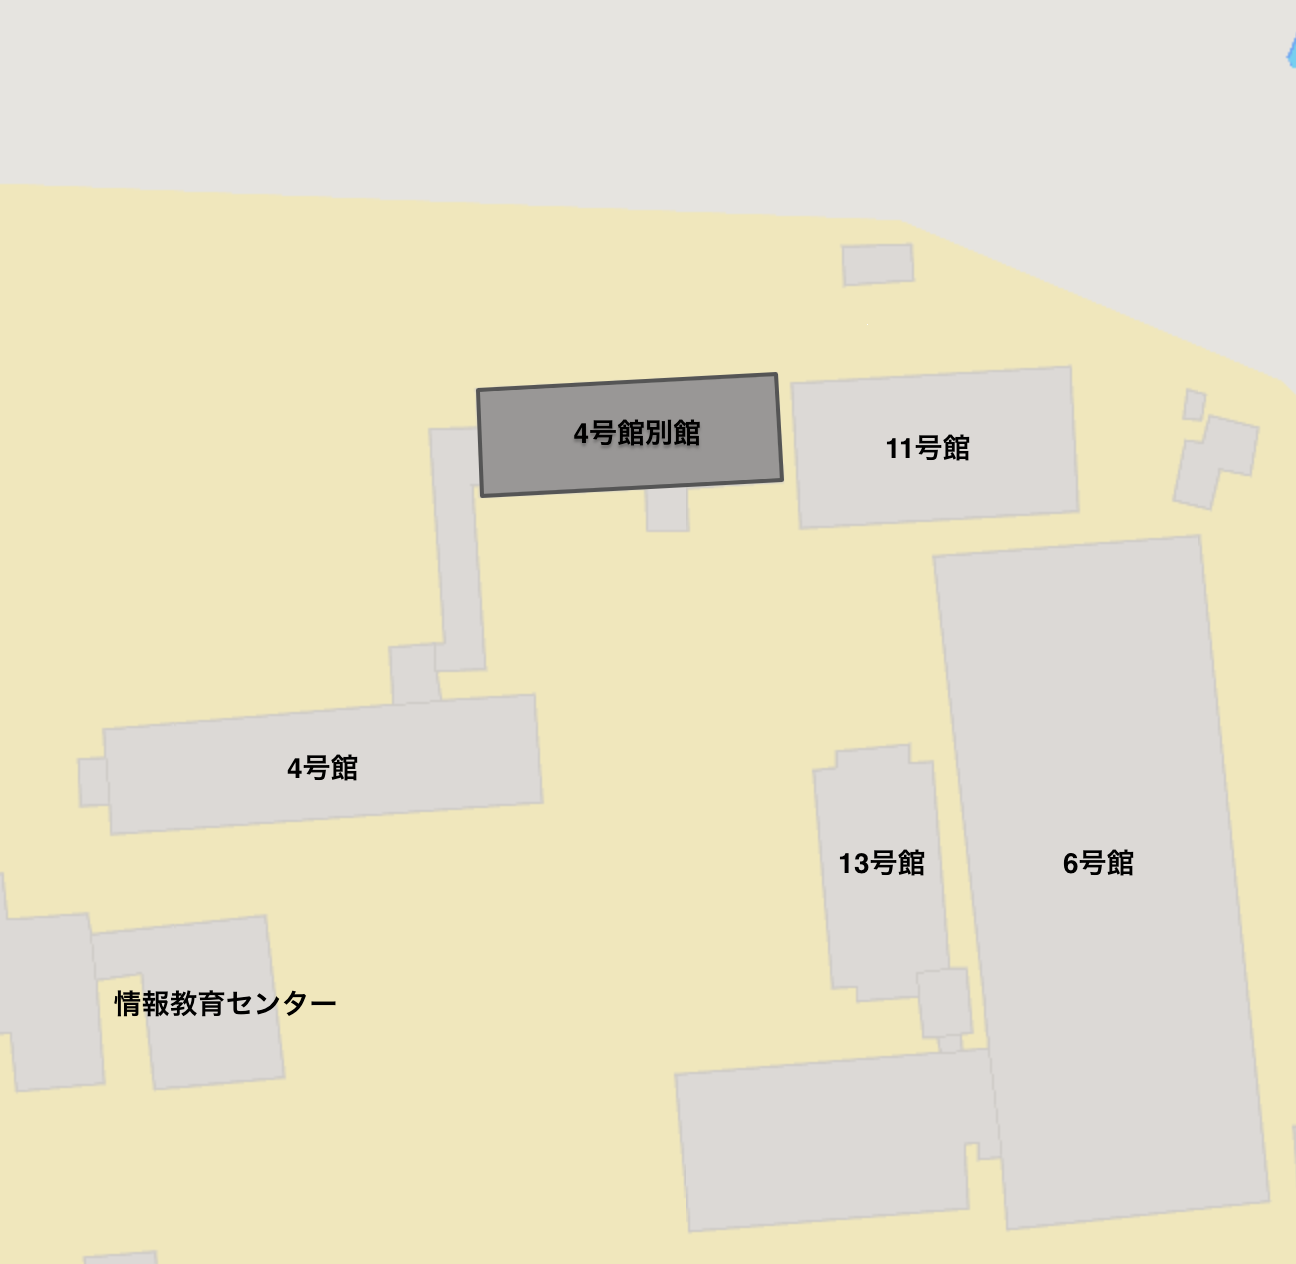
\includegraphics[width=100mm]{VerificationArea.png}
  \caption{動作検証エリア}
  \label{VerificationArea}
\end{figure}

今回の動作検証は,13時から14時までの愛知工業大学4号館別館(図\ref{VerificationArea})での活動量を加速度センサで調査するといったシナリオに基づいて行った.
スマートフォンはGoogle Pixel 4を使用した.
なお,今回の動作検証は実装の初期段階であるため,複雑な状況は想定せず,単純な状況で行う.
依頼者側は新規にWebアプリのユーザ登録を行い,協力者側は新規にスマホアプリをインストールする.
そのため,サーバには1つもセンシングプロジェクトがない状態とする.

結果として,我々が期待した通りの動作が確認できた.
まず,依頼者はWebアプリのユーザ登録を行う.

次に,Webアプリにてセンシングプロジェクトを作成する.
内容としては,時間帯を

協力者側のスマホアプリではサーバからセンシングプロジェクトを受信する.
サーバに定義された1つのセンシングプロジェクトを問題なく受信できたため,正常であると判断する.
次に,受信したセンシングプロジェクトに基づいて時空間フェンシングを行う.
指定開始時間(13時)前に動作検証エリアに進入しても通知は送られてこなかったが,指定開始時間になると通知が送られてきた.
エリアを退出するとセンシングは終了し,再度進入すると再度センシングが開始された.
エリアに進入したまま指定終了時間を迎えると,センシングは終了した.
これにより,時間判定・エリア判定ともに正常であると判断する.
動作検証エリアが屋内であるため,GPSでエリア判定を行うと位置情報誤差はあったが,動作は確認できた.屋内でのエリア判定は今後の課題とする.
また,通知も正常に送られていると確認できた.
次に,Wi-Fi接続時のみセンシングデータをアップロードする.
最初のセンシングはWi-Fiに接続していないモバイル通信の状態で終了した.
終了後にサーバを確認したところ,センシングデータは1件もなかった.
指定時間内に再度エリアに進入し,今回はWi-Fiに接続した状態でセンシングを終了した.
すると,サーバには今回のセンシングデータと最初のセンシング終了後にアップロードされなかったセンシングデータの2件が見受けられた.
Wi-Fiに接続時のみセンシングデータのアップロードは正常に確認できた.
動作検証エリアが屋内であるため,GPSでエリア判定を行うと位置情報誤差はあったが,動作は確認できた.屋内でのエリア判定は今後の課題とする.
指定した時空間内に進入すると,ヘッドアップ通知が表示され,それをタップし,依頼を承認するとセンシングが開始され,正常な動作が確認できた.
センシング後にサーバにアップロードされたセンシングデータを確認したところ,シナリオ通りに加速度が収集されていたため,動作検証は成功とする.

\begin{figure}[H]
  \centering
  \includegraphics[width=100mm]{sensingData.png}
  \caption{収集した生センシングデータ(一部)}
  \label{fig:2}
\end{figure}

% Local Variables: 
% mode: japanese-LaTeX
% TeX-master: "root"
% End: 
